% 市值变动解释性研究 — 主文档（封面 + 目录 + 章节骨架）
% 编译：xelatex main.tex（需 CJK 字体，见下方 Path）
\documentclass[UTF8, a4paper, fontset=none, zihao=-4]{ctexrep}

\usepackage{fontspec}
\newcommand{\WinFonts}{/mnt/c/Windows/Fonts/}
\setCJKmainfont{simsun.ttc}[Path=\WinFonts, BoldFont=simhei.ttf, ItalicFont=simkai.ttf]
\setCJKsansfont{simhei.ttf}[Path=\WinFonts, BoldFont=simhei.ttf]
\setCJKmonofont{simfang.ttf}[Path=\WinFonts]

\usepackage{geometry}
\geometry{margin=2.6cm}
\usepackage{amsmath}
\usepackage{amssymb}
\usepackage{graphicx}
\usepackage{booktabs}
\usepackage{tabularx}
\usepackage{xcolor}
\usepackage{colortbl}
\usepackage{longtable}
\usepackage{needspace}
\usepackage{caption}
\usepackage{fancyhdr}
\usepackage{titlesec}
\usepackage{tikz}
\usetikzlibrary{arrows.meta, positioning}
\usepackage{float}
\usepackage{microtype}
\setlength{\headheight}{15pt}

% —— 版式：行距更舒展、浮动体与正文留白更从容 ——
\linespread{1.25}
\setlength{\parskip}{0pt plus 1pt}
\setlength{\textfloatsep}{20pt plus 3pt minus 3pt}
\setlength{\floatsep}{16pt plus 3pt minus 3pt}
\setlength{\intextsep}{18pt plus 3pt minus 3pt}
\setlength{\abovecaptionskip}{8pt}
\setlength{\belowcaptionskip}{2pt}
% 浮动体放置：更愿意用正文填满页面、图表落到页顶/底，减少大片留白
\renewcommand{\topfraction}{0.92}
\renewcommand{\bottomfraction}{0.85}
\renewcommand{\textfraction}{0.08}
\renewcommand{\floatpagefraction}{0.72}
\setcounter{topnumber}{2}
\setcounter{bottomnumber}{1}
\setcounter{totalnumber}{3}

% 品牌色（与插图配色一致）
\definecolor{brandblue}{HTML}{2F6DB5}
\definecolor{brandred}{HTML}{D8443C}
\definecolor{ink}{HTML}{22303F}
\definecolor{brandgreen}{HTML}{2E8B6F}
\definecolor{okbg}{HTML}{DCEDE5}
\definecolor{nobg}{HTML}{F7DCD4}

\captionsetup{font={small, color=ink}, labelfont={bf, color=brandblue}, labelsep=quad,
              justification=raggedright, singlelinecheck=false, skip=7pt}
\graphicspath{{../figures/ml_report/}}

% 页眉页脚：细线、低饱和，含蓄而正式
\pagestyle{fancy}
\fancyhf{}
\fancyhead[L]{\footnotesize\color{brandblue} 市值变动解释性研究}
\fancyhead[R]{\footnotesize\color{brandblue}\leftmark}
\fancyfoot[C]{\small\color{ink}\thepage}
\renewcommand{\headrulewidth}{0.3pt}
\renewcommand{\headrule}{{\color{brandblue!35}\hrule height \headrulewidth}\vspace{-\headrulewidth}}

% 章标题：不另起页、接排；小号灰色"第 X 章"题眉 + 大号标题 + 细分隔线
\titleclass{\chapter}{straight}
\titleformat{\chapter}[display]
  {\needspace{7\baselineskip}\sffamily\bfseries\color{ink}}
  {\fontsize{15}{18}\selectfont\color{brandblue}\sffamily 第\,\thechapter\,章}
  {8pt}{\fontsize{24}{30}\selectfont}[{\vspace{9pt}\color{brandblue}\titlerule[1.1pt]}]
\titlespacing*{\chapter}{0pt}{28pt plus 6pt minus 4pt}{20pt}
\setcounter{tocdepth}{0}   % 目录只列到章，避免节标题撑溢出
% 节标题：左对齐、加粗、品牌色
\titleformat{\section}
  {\sffamily\bfseries\color{ink}\large}{\color{brandblue}\thesection}{0.7em}{}
\titlespacing*{\section}{0pt}{*2.7}{*1.25}

\begin{document}

% ============ 封面 ============
\begin{titlepage}
\centering
\thispagestyle{empty}
\vspace*{2.6cm}
% 研究主体题眉
{\sffamily\color{ink}\fontsize{13}{17}\selectfont 移为通信（300590）及可比同业\par}
\vspace{0.45cm}
{\color{brandblue}\rule{2.4cm}{1pt}\par}
\vspace{1.7cm}
% 主标题
{\sffamily\bfseries\color{ink}\fontsize{36}{44}\selectfont 市值变动的解释性研究\par}
\vspace{1.05cm}
{\sffamily\color{brandblue}\fontsize{15.5}{24}\selectfont 基于面板数据的稳健推断\\[3pt]与机器学习描述性归因\par}
\vspace{2.7cm}
% 细线之间的研究元信息
{\color{brandblue}\rule{0.86\textwidth}{0.7pt}\par}
\vspace{0.85cm}
{\color{ink}\fontsize{11.5}{15}\selectfont
\begin{tabular}{@{}r@{\hspace{1.4em}}l@{}}
{\sffamily\bfseries\color{brandblue}研究主体} & 移为通信 ＋ 13 家纯模组 / 终端可比公司\\[7pt]
{\sffamily\bfseries\color{brandblue}研究命题} & 解释市值为何变动（非预测股价）\\[7pt]
{\sffamily\bfseries\color{brandblue}方\hspace{2em}法} & 恒等分解 ＋ 面板/少簇稳健推断 ＋ 机器学习描述性归因\\
\end{tabular}\par}
\vspace{0.85cm}
{\color{brandblue}\rule{0.86\textwidth}{0.7pt}\par}
\vfill
{\color{ink}\fontsize{11}{16}\selectfont 2026 年 6 月\par}
\vspace{0.8cm}
\end{titlepage}

% ============ 执行摘要 ============
\thispagestyle{fancy}
{\linespread{1.07}\selectfont
\vspace*{0.02cm}
{\sffamily\bfseries\color{ink}\fontsize{23}{28}\selectfont 摘要\par}
\vspace{7pt}{\color{brandblue}\rule{\textwidth}{1.1pt}\par}
\vspace{11pt}

本报告解释移为通信及 13 家可比公司的市值\emph{为何}有高有低——把估值差异归到可解释的经营基本面上，而非预测股价。主要发现如下。

\vspace{7pt}
\noindent{\sffamily\bfseries\color{brandblue}三条全样本规律}
\begin{enumerate}\setlength{\itemsep}{2pt}\setlength{\parskip}{0pt}\setlength{\topsep}{2pt}
\item \textbf{负债越低，市场给的估值越高。}14 家中证据最强、最稳健的规律，多种独立检验一致成立。
\item \textbf{营收增长越快，估值倍数反而被压低。}与“规模扩张即享溢价”的常识相反——该赛道对单纯的规模扩张给折价、而非溢价。
\item \textbf{盈利能力（利润率）对估值无可靠影响。}以短期利润率提升估值，数据不支持。
\end{enumerate}
并且，\textbf{基本面只能解释这些公司估值差异的约一半}；另一半来自市场情绪与叙事等无法由基本面衡量的因素，故只看基本面的估值判断天然带约一半不确定。

\vspace{7pt}
\noindent{\sffamily\bfseries\color{brandblue}移为通信诊断}\par
移为当前的估值溢价，\textbf{约一半有基本面支撑}（主要来自其显著低于同业的负债水平），\textbf{另一半由情绪驱动、并不牢靠}；前者可持续，后者随市场预期回摆。移为真正扎实的估值优势是“低负债”这一条，其余溢价存在回调风险。

\vspace{7pt}
\noindent{\sffamily\bfseries\color{brandblue}对决策的含义}
\begin{itemize}\setlength{\itemsep}{2pt}\setlength{\parskip}{0pt}\setlength{\topsep}{2pt}
\item \textbf{杠杆——唯一可操作的稳健驱动：}资产负债率与超额估值稳健负相关、且为公司可控协变量；维持低杠杆为移为可持续的估值优势来源，宜列为重点维持的财务指标。
\item \textbf{成长——真实但非正向抓手：}营收增长与估值倍数稳健负相关；增长叙事宜以质量、而非规模为支点。
\item \textbf{情绪敞口：}约半数溢价为与基本面正交的特异/情绪成分，构成模型外的不确定性敞口，宜单列并预留回撤空间。
\end{itemize}

\vspace{7pt}
\noindent{\sffamily\bfseries\color{brandblue}经检验不构成估值驱动的因素（噪音，供参考）}
\begin{itemize}\setlength{\itemsep}{2pt}\setlength{\parskip}{0pt}\setlength{\topsep}{2pt}
\item \textbf{盈利能力（利润率）：}偏效应未通过稳健性检验、公司内估计变号；且检验功效不足，故为未获稳健支持、而非已证明无关。
\item \textbf{资本运作与公告事件}（并购重组、定增、员工持股等）：经市场模型事件研究核对无稳健方向性异常收益，同窗口事件重叠难归因。
\item \textbf{文本与舆情信号}（披露文本、互动问答、新闻、研报）：预测信息系数约 $0.14$，弱信号，已剔除。
\item \textbf{市场结构与筹码、及 L1 剔除的冗余指标}（北向持股、融资余额、换手率等市场结构特征，连同 L1 剔除的 $25$ 项高共线/弱信号特征）：含市值机械成分、稳定性低，或信息已被保留特征覆盖，均属关联层、非稳健驱动。
\end{itemize}

\vspace{6pt}
以上为方向性结论（量级而非精确点估计，宜作决策依据之一）；完整方法、数据与稳健性检验见正文各章与附录。
\par}
\clearpage

% ============ 目录 ============
\tableofcontents
\thispagestyle{fancy}
\clearpage

% ============ 正文章节骨架（占位，逐章填充）============
\chapter{引言与命题}

\section{研究命题}
本报告旨在\textbf{解释}移为通信及其可比同业的市值\emph{为何}变动——把市值在公司间与时间上的差异归因到可解释的基本面驱动；而\textbf{非预测}未来股价。二者在统计目标上根本不同：解释关注条件期望 $\mathbb{E}[Y\mid X]$ 的结构与各驱动的贡献。鉴于样本仅 $14$ 家公司、有效独立簇更少（详见第\ref{ch:limitations}章），本报告的可信推断不依赖灵活模型的样本内拟合，而是以面板/公司内回归配合少簇稳健方法为主干；机器学习模型只作描述性归因，其解释力一律以\emph{样本外}（留一家、留时段）$R^2$ 衡量，不报样本内 $R^2$。预测关注对未实现价格的外推，在本问题中受制于低信噪比与过拟合（详见第\ref{ch:limitations}章），故本报告仅将预测作为如实标注不确定性的\emph{建议层}，不作主张。

\section{恒等分解框架}
任一主体的市值满足恒等式
\[
  \text{市值} \;=\; \text{营收} \times \underbrace{\frac{\text{市值}}{\text{营收}}}_{\text{市销率 PS}} \;=\; \text{营收} \times \text{PS},
\]
即市值由\textbf{营收规模}（经营基本面）与\textbf{每元营收的市场定价}（估值倍数 PS）两部分构成。本报告全部分析都沿这一分解展开：市值变动先归入\emph{经营通道}与\emph{估值再定价通道}，再追问各通道由哪些基本面驱动、是否稳健。

\section{对数变换}
上式是相乘关系，无法直接分配“营收与估值各贡献多少”。取对数把相乘变为相加——$\ln(\text{市值})=\ln(\text{营收})+\ln(\text{PS})$——市值变动便可精确拆为经营通道与估值再定价通道之和（图~\ref{fig:spine}）。这是分解框架成立的前提。

取对数还带来两点便利：对数差近似等于百分比变化（如 $+10\%$ 对应 $\Delta\ln\approx0.1$），与市值以涨跌幅衡量的习惯一致；且市值、营收为右偏分布，取对数后更接近对称、更适合线性回归。


\begin{figure}[htbp]
\centering
\begin{tikzpicture}[
  box/.style={draw=brandblue, line width=1pt, rounded corners=4pt, align=center,
              inner sep=9pt, font=\sffamily, minimum width=\linewidth},
  arr/.style={-{Stealth[length=3mm]}, line width=1pt, color=ink},
]
\node[box] (a) {市值 \;=\; 营收 \;$\times$\; 估值倍数\,(PS)\\[2pt]
  {\footnotesize\color{ink!65} 乘性恒等：贡献不可直接分配}};
\node[box, below=15mm of a] (b) {$\ln(\text{市值}) \;=\; \ln(\text{营收}) \;+\; \ln(\text{PS})$\\[2pt]
  {\footnotesize\color{ink!65} 加性结构：可分解为独立通道}};
\node[box, below=15mm of b] (c) {%
  $\Delta\ln(\text{市值}) \;=\; \underbrace{\Delta\ln(\text{营收})}_{\text{经营通道}}
  \;+\; \underbrace{\Delta\ln(\text{PS})}_{\text{估值再定价通道}}$\\[2pt]
  {\footnotesize\color{ink!65} 两通道之和 $\equiv$ 总变动（精确分解）}};
\draw[arr] (a) -- node[right, font=\small\sffamily]{\;取对数：相乘 $\to$ 相加} (b);
\draw[arr] (b) -- node[right, font=\small\sffamily]{\;取变动（差分）} (c);
\end{tikzpicture}
\caption{市值的恒等分解脊柱：乘性恒等经对数变换转为加性，市值变动精确分解为经营通道与估值再定价通道。}
\label{fig:spine}
\end{figure}

\section{报告结构}
本报告以恒等分解脊柱为组织主线：各章围绕“任一市值变动先归入经营通道与估值再定价通道、再追问其基本面来源”展开，分为六个阶段（表~\ref{tab:roadmap}）。全报告的分工是：可信推断以面板/公司内回归配合少簇稳健方法为主干，机器学习模型只作描述性归因。

\begin{table}[htbp]
\caption{报告结构：六个阶段及其主要内容}
\label{tab:roadmap}
\renewcommand{\arraystretch}{1.35}
\begin{tabularx}{\textwidth}{@{}l l X@{}}
\toprule
\textbf{\color{brandblue}阶段} & \textbf{\color{brandblue}章次} & \textbf{\color{brandblue}主要内容} \\
\midrule
数据与目标 & 第 2--3 章 & 样本界定与时点对齐面板；超额估值目标变量的构造 \\
特征 & 第 4--6 章 & 探索性分析、防泄漏特征工程、算术耦合审查与 L1 特征选择 \\
建模与调参 & 第 7--8 章 & 浅树梯度提升树与白盒线性的描述性建模；嵌套交叉验证调参 \\
验证 & 第 9 章 & 样本外与留一家验证；解释力上限的界定 \\
描述与推断 & 第 10--11 章 & SHAP 描述性归因与稳定性区间；面板/公司内回归＋少簇稳健的推断主干 \\
结论 & 第 12--13 章 & 全域规律、逐家诊断与决策剪枝；局限与有效性威胁 \\
\bottomrule
\end{tabularx}
\end{table}

\chapter{数据与样本}\label{ch:data}
要解释跨公司的市值差异，前提是一个口径可比、且不含前视信息的面板。本章依次交代数据来源、样本范围与面板结构。

\section{数据来源}
本报告的数据分为两类。\textbf{进入模型的量化数据}全部来自 Tushare，涵盖财务指标、三大报表、每日市值与市销率、主营业务构成、北向持股、融资融券、资金流向、股东户数与前十大流通股东；各项均带公告日时间戳，为时点对齐提供依据（接口清单见附录~\ref{app:repro}）。

项目另\textbf{采集但未纳入模型}的数据，包括巨潮资讯的披露报告与互动易问答、东方财富的公告、研究报告、新闻与机构调研。这些披露与文本数据曾被加工为事件候选与文本派生的非财务信号特征，分别用于事件研究线与预测线；二者经检验为噪声（事件后 20 日异常反应 $R^2<0$）与弱信号（信息系数约 $0.14$），均已废弃。因此本报告的估值模型仅使用上述 Tushare 量化数据，不含任何文本或舆情信号。

\section{样本范围}
为使估值横向可比，本报告将样本限定为纯模组与终端公司，共 14 家（表~\ref{tab:firms}）。上游半导体与芯片设计、定位导航整机、以及软件与运维服务类公司，因业务层级或商业模式不同、估值逻辑相异，未纳入样本。

\begin{table}[htbp]
\caption{研究样本：14 家纯模组与终端可比公司（移为通信为研究主体）}
\label{tab:firms}
\renewcommand{\arraystretch}{1.3}
\begin{tabular*}{\textwidth}{@{\extracolsep{\fill}}llllll@{}}
\toprule
\textbf{\color{brandblue}公司} & \textbf{\color{brandblue}代码} & \textbf{\color{brandblue}板块}
 & \textbf{\color{brandblue}公司} & \textbf{\color{brandblue}代码} & \textbf{\color{brandblue}板块}\\
\midrule
日海智能 & 002313 & 深主板 & 广和通 & 300638 & 创业板\\
金溢科技 & 002869 & 深主板 & 博实结 & 301608 & 创业板\\
美格智能 & 002881 & 深主板 & 移远通信 & 603236 & 沪主板\\
锐明技术 & 002970 & 深主板 & 映翰通 & 688080 & 科创板\\
高新兴 & 300098 & 创业板 & 有方科技 & 688159 & 科创板\\
万集科技 & 300552 & 创业板 & 三旺通信 & 688618 & 科创板\\
\textbf{移为通信} & \textbf{300590} & 创业板 & 利尔达 & 920249 & 北交所\\
\bottomrule
\end{tabular*}
\end{table}

\section{面板结构与覆盖}
面板的观测单元为“公司–报告期”，报告期为季度频率（季报、半年报与年报），共 483 个观测，覆盖 14 家公司、2009 至 2026 年。每个观测包含 42 个候选特征，涵盖盈利与现金流质量、运营效率、杠杆与流动性、成长性、费用与研发、海外业务，以及市场流动性与筹码等类别（特征定义与口径见附录~\ref{app:datadict}）。财务数据按公告日以最近可得值对齐至各报告期，避免前视偏误；时点对齐的具体做法详见第\ref{ch:feature}章。

面板为非平衡结构：各公司上市时点不同，历史长度差异显著（图~\ref{fig:panel}）。历史最长者（日海智能、高新兴）覆盖 60 余个报告期，而次新股（如博实结仅 9 期）样本极短；横截面上具备完整历史的公司不足半数。这一差异源于行业内公司上市集中于 2016 年之后，早期可比样本稀缺。

非平衡结构对建模有两点直接影响。其一，以公司为单位的有效样本仅 14 家，远小于特征数，存在“维数高于样本”的过拟合风险——这是后续必须做特征选择与正则化、并采用深度受限模型的根本原因。其二，留一家外推验证在历史较短的公司上方差更大，其外推结论须谨慎解读。两点共同决定了本报告“以可解释、强约束模型换取稳健性”的建模取向。

\begin{figure}[htbp]
\centering
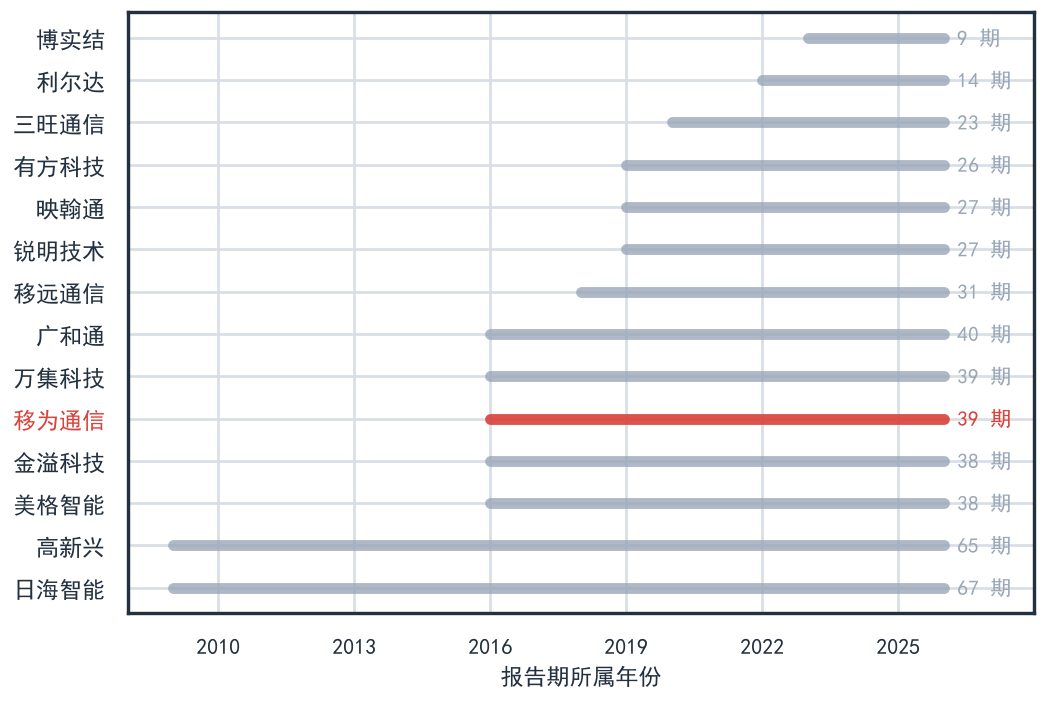
\includegraphics[width=\textwidth]{F2_面板覆盖时间线.png}
\caption{14 家公司的报告期覆盖（非平衡面板）。横条为各公司可用报告期的时间跨度，行尾数字为期数，移为通信以红色标注；历史最长者（日海智能、高新兴）逾 60 期，次新股（博实结仅 9 期）样本极短。}
\label{fig:panel}
\end{figure}

\chapter{目标变量构造}
本章构造解释对象——目标变量 $Y$。直接用市销率无法回答“某公司估值为何偏高或偏低”，因为市销率中混入了与公司特异定价无关的共同成分。本章先剖解这些成分，再逐项剥离，得到\emph{超额估值}作为目标。

\section{原始市销率的混淆成分}
同一时点不同公司的市销率（PS，市值与营收之比）不可直接横向比较，因为它至少包含三部分：

\begin{enumerate}
  \item \textbf{逐年的行业估值水位}：整个赛道的估值随市场与板块周期逐年同涨同跌。2021 年所有公司的市销率都高、2023 年都低，这一共同水位与单家公司的优劣无关。
  \item \textbf{规模效应}：市值规模不同的公司，市场赋予的倍数系统性不同（通常大市值公司倍数更高或更稳）。
  \item \textbf{公司特异的溢价或折让}：剥掉上述两者后，真正反映“这家公司比同规模、同年份的同行贵或便宜多少”的部分——这正是本报告要解释的对象。
\end{enumerate}

\section{超额估值的构造}
超额估值衡量一家公司相对\textbf{同年同行}的高估或低估，分两步从对数市销率中剥离共同成分。

\textbf{第一步，减去当年行业水位。} 当年行业水位即该年全部公司对数市销率的平均。以 2023 年为例，14 家公司当年的对数市销率列于表~\ref{tab:logps2023}：把这 14 个数相加除以 14，得平均 \textbf{1.17}，这就是 2023 年的行业估值水位。移为通信当年为 \textbf{1.64}，高出行业水位 $1.64-1.17=\textbf{0.47}$。

\begin{table}[htbp]
\centering
\caption{2023 年 14 家公司的对数市销率（移为通信加粗；其 14 家平均即当年行业水位 $1.17$）}
\label{tab:logps2023}
\renewcommand{\arraystretch}{1.25}
\begin{tabular}{l r @{\hspace{2.6cm}} l r}
\toprule
\textbf{\color{brandblue}公司} & \textbf{\color{brandblue}对数市销率} & \textbf{\color{brandblue}公司} & \textbf{\color{brandblue}对数市销率}\\
\midrule
三旺通信 & 2.45 & 锐明技术 & 1.25\\
金溢科技 & 1.94 & 美格智能 & 1.10\\
映翰通 & 1.93 & 高新兴 & 1.05\\
博实结 & 1.73 & 广和通 & 0.90\\
\textbf{移为通信} & \textbf{1.64} & 日海智能 & $-0.06$\\
万集科技 & 1.56 & 移远通信 & $-0.09$\\
有方科技 & 1.34 & 利尔达 & $-0.38$\\
\bottomrule
\end{tabular}
\end{table}

\begin{figure}[htbp]
\centering
\begin{tikzpicture}[
  box/.style={draw=brandblue, line width=1pt, rounded corners=4pt, align=center,
              inner sep=9pt, font=\sffamily, minimum width=\linewidth},
  arr/.style={-{Stealth[length=3mm]}, line width=1pt, color=ink},
]
\node[box] (a) {移为通信 2023 年｜市销率 ＝ 市值 ÷ 营收\\[2pt]
  {\footnotesize\color{ink!65} 衡量每元营收市场愿付的价}};
\node[box, below=6mm of a] (b) {取对数后，对数市销率 ＝ \textbf{1.64}\\[2pt]
  {\footnotesize\color{ink!65} 取对数便于加减比较}};
\node[box, below=6mm of b] (c) {减去当年行业水位 \textbf{1.17}（14 家平均）：\;$1.64-1.17=\textbf{0.47}$\\[2pt]
  {\footnotesize\color{ink!65} 去掉全行业当年的共同涨跌}};
\node[box, below=6mm of c] (d) {按规模微调（移为规模接近行业平均，调整 $\approx 0$），得 2023 年\textbf{超额估值} $\approx 0.47$\\[2pt]
  {\footnotesize\color{ink!65} 各报告期平均 $+0.70$（早年溢价更高），处于明显溢价}};
\draw[arr] (a) -- (b);
\draw[arr] (b) -- (c);
\draw[arr] (c) -- (d);
\end{tikzpicture}
\caption{以移为通信 2023 年为例的超额估值计算：对数市销率 $1.64$，减去当年 14 家平均水位 $1.17$ 得 $0.47$，再按规模微调（移为几乎不变），所得即超额估值。}
\label{fig:target}
\end{figure}

\textbf{第二步，剥离规模影响。} 规模是估值的标准控制项，故在剥离行业水位的同一回归中再纳入对数市值。具体做法是把 14 家公司全样本的对数市销率，对\emph{对数市值}与\emph{年度哑变量}一并做最小二乘拟合，对数市值那一项的系数即\textbf{规模系数 $-0.05$}：在同一年份内，对数市值每高 $1$ 个单位（体量约大 $2.7$ 倍），对数市销率仅低约 $0.05$。事实上，本样本中对数市值与对数市销率的线性相关系数仅为 $-0.05$，二者\textbf{几乎不相关}——对数市值从最小 $11.8$ 到最大 $14.9$ 跨越约 $3$ 个单位，对应的估值差异也不过约 $0.17$。因此这一步对所有公司都只是小幅修正。这一点在图~\ref{fig:size} 中清晰可见：把全部观测按规模从小到大分为 $6$ 档，各档剥离年度后的对数市销率平均值基本落在同一水平，最大相差仅 $0.26$，置信区间彼此重叠，可见规模几乎不影响估值倍数。移为通信处于中等规模的第 $4$ 档（其对数市值约 $13.20$，接近样本均值 $13.19$），规模调整约为 $-0.0002$，可忽略；其超额估值基本等于第一步剥离当年行业水位后的偏离。

\begin{figure}[htbp]
\centering
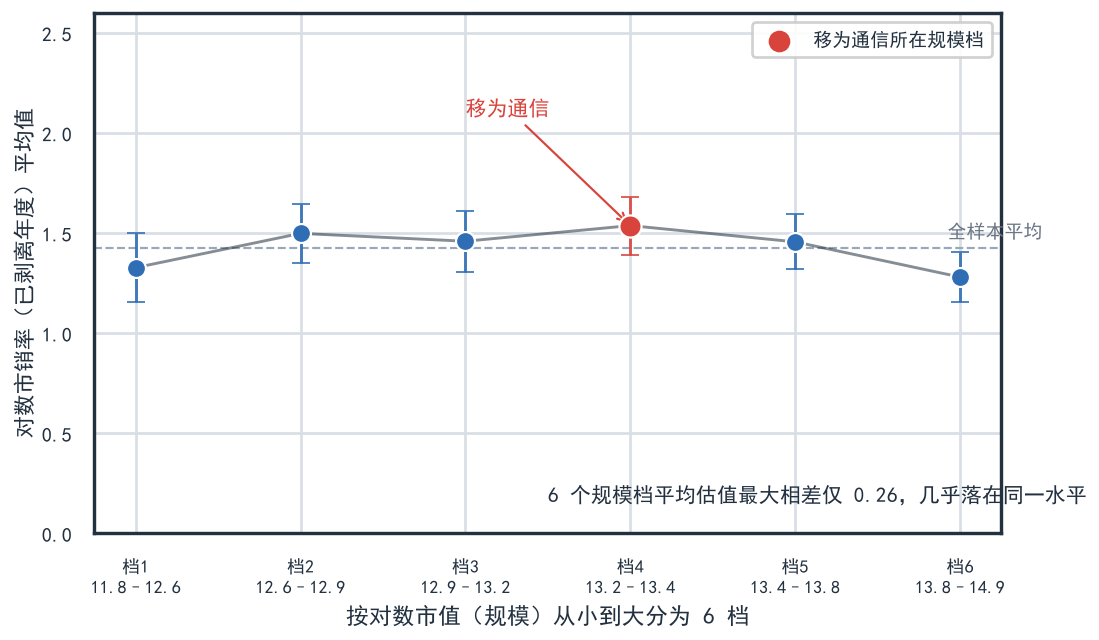
\includegraphics[width=\textwidth]{F_规模效应.png}
\caption{规模对估值倍数的影响（分档平均）。按对数市值（规模）从小到大分为 $6$ 档，每档约 $80$ 个观测；圆点为该档剥离年度后的对数市销率均值，竖线为 $95\%$ 置信区间，横虚线为全样本平均。六档均值最大相差仅 $0.26$、基本落在同一水平，表明规模与估值倍数几乎无关。移为通信位于中等规模的第 $4$ 档（红点），故规模调整约为零。}
\label{fig:size}
\end{figure}

把上述两步用于移为的每个报告期并取平均，其超额估值约 \textbf{$+0.70$}（2023 年为 $0.47$，早年溢价更高，故均值更大），处于明显溢价一侧（对数市销率先按 $2\%/98\%$ 分位缩尾以抑制极端值）。

\section{目标分布与解读}
由于每期都剥离了当年行业水位与规模影响，$Y$ 的样本均值约为零、标准差为 $0.68$。$Y$ 为正表示该公司相对同规模、同年份同行存在估值溢价，为负则为折让。图~\ref{fig:targethist} 按公司均值排序，逐家展示各公司的平均超额估值：每行一家公司，圆点为其平均 $Y$，横线为 $95\%$ 置信区间，竖虚线为同年份、同规模同行的水位基准。研究主体移为通信的平均超额估值为 $+0.70$，在 14 家中位列次高，处于明显溢价一侧；同为模组厂的移远通信、利尔达则处于折让一侧。这一跨公司的溢价差异由何驱动，正是后续特征建模要回答的问题。需说明，$Y$ 是第一阶段回归（对数市销率对规模与年度）的\emph{残差}，本身是估计量、而非直接观测的真值；因此后续推断不把它当作已知真值，而是通过对整条管线（含这一第一阶段）重抽样，把这一步的估计不确定性也一并纳入（详见稳健性与推断一章）。

\begin{figure}[htbp]
\centering
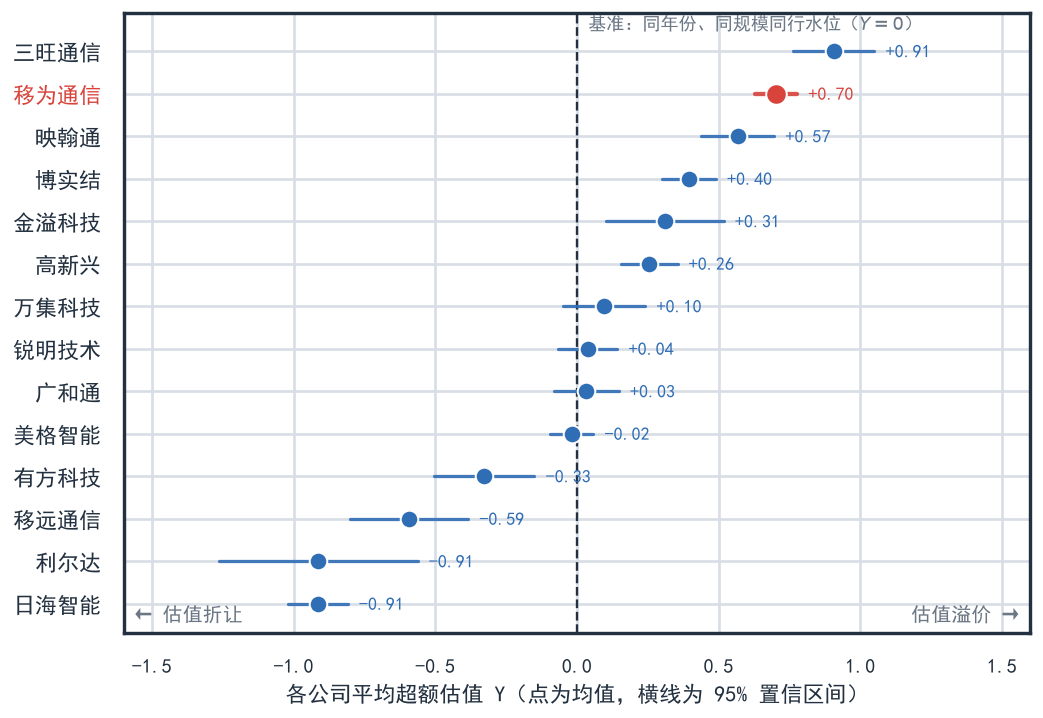
\includegraphics[width=0.72\textwidth]{F3_目标变量分布.png}
\caption{各公司平均超额估值 $Y$（按均值升序排列）。每行一家公司，圆点为其平均 $Y$、横线为 $95\%$ 置信区间，竖虚线为同年份、同规模同行的水位基准（$Y=0$）：右侧为估值溢价、左侧为折让。移为通信平均 $+0.70$、位列次高；全样本均值约 $0$、标准差 $0.68$。}
\label{fig:targethist}
\end{figure}

分布大致对称，正负两侧观测数相当——约半数公司–报告期为溢价、半数为折让，说明同一行业内估值分化显著，并非所有公司都被一致定价。移为通信稳居溢价一侧（平均 $+0.70$），但这一溢价由哪些基本面驱动、是否可持续，无法从分布本身回答，须引入特征建模。

至此目标变量构造完毕。后续要用一组基本面与市场特征来解释 $Y$，但这些特征能否直接进入回归，取决于它们彼此的相关结构与数据质量。下一章先对特征做探索性分析，据此确定建模前必须采取的处理。

\chapter{探索性数据分析}\label{ch:eda}

\section{高维小样本的处境}
建模样本为 $483$ 个“公司—报告期”观测，来自 $14$ 家公司、覆盖 $2009$ 至 $2026$ 年。候选特征共 $42$ 个，即第\ref{ch:data}章面板中的全部指标，涵盖盈利与现金流质量、运营效率、杠杆与流动性、成长性、费用与研发、海外业务及市场微结构等类别，逐项定义与计算口径见附录~\ref{app:datadict}；本章用到的净利率、毛利率、研发强度、资产负债率、ROE 等均出自这一候选集。这一规模存在三重不利：特征数与样本量之比偏高（$42$ 对 $483$）；观测按公司成簇，$14$ 家各贡献数十期、簇内高度相关，独立信息量远小于表面数字；二者叠加使灵活模型极易记住偶然波动而非普遍规律，造成过拟合且系数不稳。因此在建模前先做诊断性的探索性数据分析，识别会损害模型稳定性与可解释性的结构性问题，并据此确定预处理与建模策略——每一项诊断都对应一个具体的建模决策。本章依次检视三类问题：特征间的强共线性、分布偏态与极端值、缺失结构。

\section{特征间的强共线性}\label{sec:collinear}
基本面指标之间并非彼此独立，许多指标在定义上或经济含义上高度重叠。图~\ref{fig:corr} 给出上述候选特征中核心基本面指标两两之间的皮尔逊相关系数（即标准化后的协方差，取值在 $[-1,1]$，对角线恒为 $1$）：净利率与营业利润率高达 $0.99$，二者近乎同一变量；资产负债率与现金比率为 $-0.77$、与毛利率为 $-0.72$，毛利率与现金比率为 $0.67$——盈利能力指标、杠杆与流动性指标各自构成一个高度共线的族。

\begin{figure}[htbp]
\centering
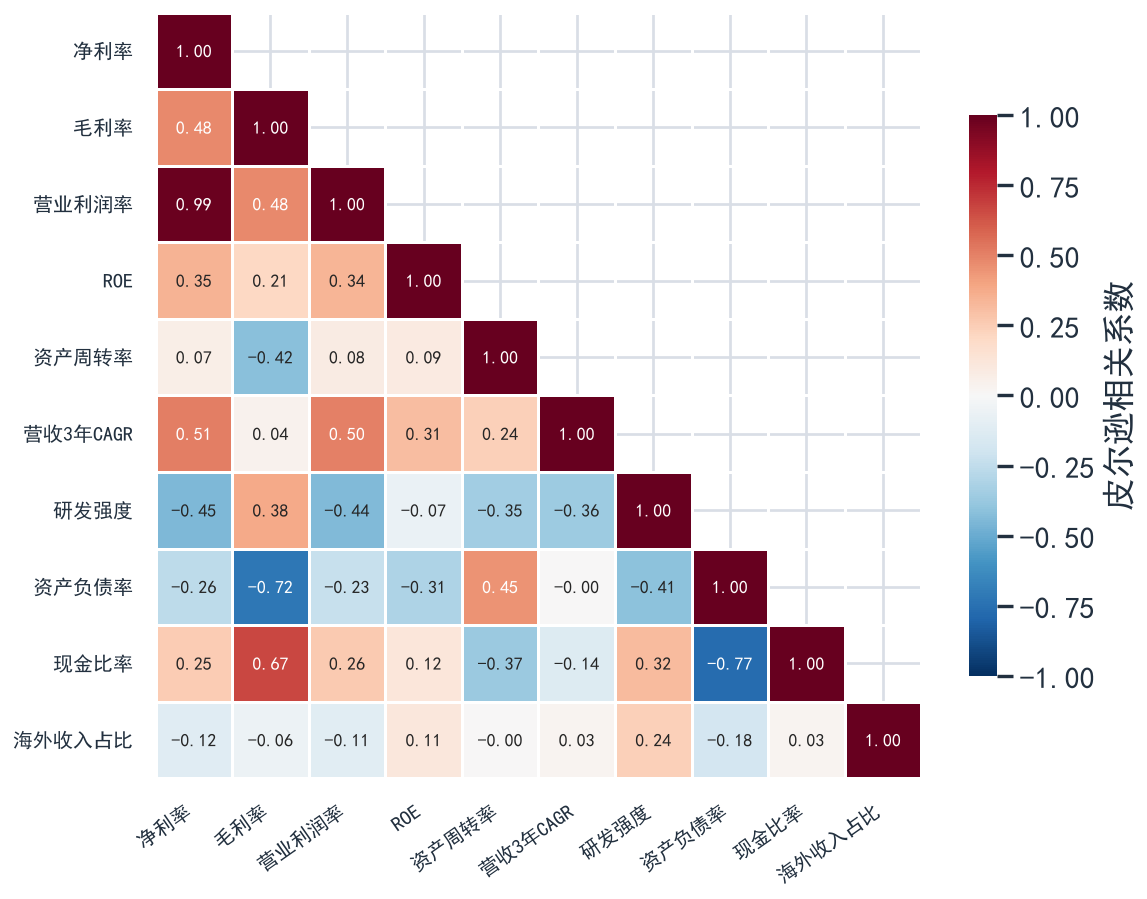
\includegraphics[width=0.70\textwidth]{F4_特征相关矩阵.png}
\caption{核心基本面特征的两两皮尔逊相关系数（下三角，颜色越深相关越强）。净利率与营业利润率高达 $0.99$、近乎同一变量；资产负债率与现金比率 $-0.77$、与毛利率 $-0.72$，毛利率与现金比率 $0.67$，显示盈利能力、杠杆与流动性指标各自高度共线。}
\label{fig:corr}
\end{figure}

强共线性会从两个方向损害模型。对无约束的线性模型，它使系数在相互关联的特征之间被任意分配：单个特征的系数大小不稳、符号可能随样本的微小扰动而反转，于是无法回答“究竟是哪一项在驱动估值”。对灵活的树模型，它使模型在近乎重复的特征之间反复分裂，放大方差、削弱泛化。这正是不能把 $42$ 个特征直接全部输入一个灵活模型的首要理由。

针对性的处理放在后续两章：特征选择一章以 L1（Lasso）正则化从每个共线族中保留代表、将冗余特征的系数压至零；建模一章只对个别方向有强先验且经独立验证的特征（如资产负债率）施加单调约束，其余特征不约束、由数据决定方向。共线性因此由潜在隐患转为被显式处理的环节。

\section{分布偏态与极端值}\label{sec:skew}
第二类问题是特征分布显著偏离对称、并含极端观测。图~\ref{fig:skew} 给出与图~\ref{fig:corr} 相同的一组核心基本面指标的偏度系数（偏度为分布对称性的标准度量）：研发强度（$+2.3$）、现金比率（$+1.6$）、资产周转率（$+1.3$）呈明显右偏（长右尾），净利率（$-1.3$）、营业利润率（$-1.2$）呈左偏；其中 ROE 的偏度低至 $-9.7$，远在近似对称区 $[-1,1]$ 之外，意味着分布被个别极端观测主导——例如个别年份的巨额亏损会令净资产收益率出现极端取值。

\begin{figure}[htbp]
\centering
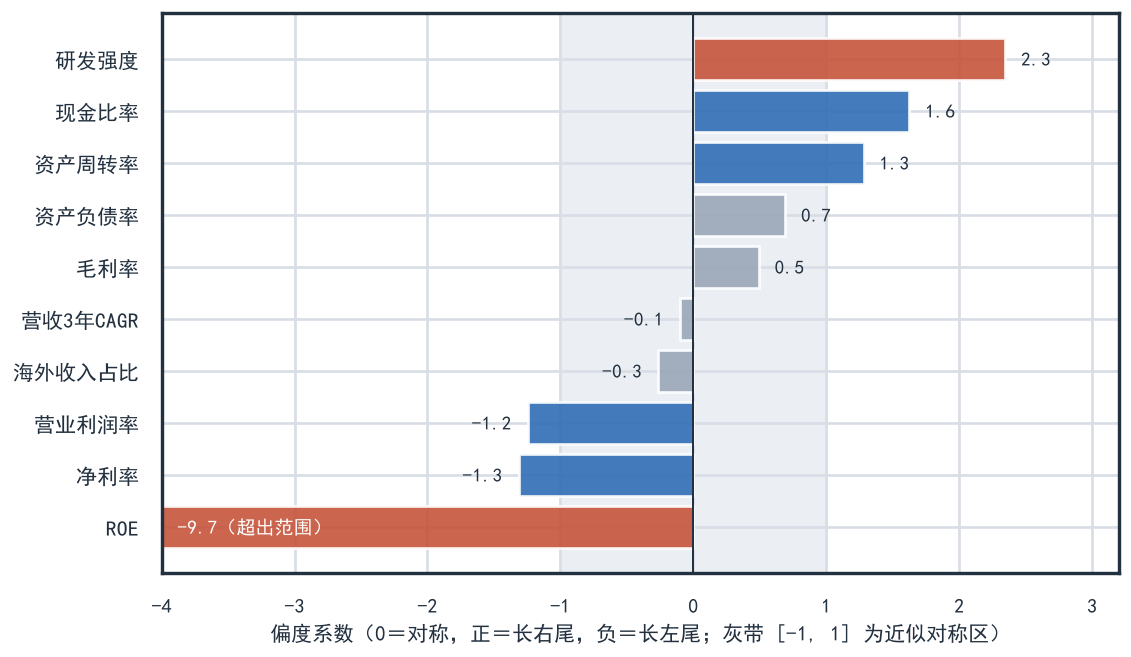
\includegraphics[width=\textwidth]{F6_特征偏态体检.png}
\caption{核心特征的偏度系数（$0$ 为对称，正值表示长右尾、负值表示长左尾；灰带 $[-1,1]$ 为近似对称区）。多数特征落在对称区之外，研发强度偏度 $+2.3$、ROE 低至 $-9.7$（超出坐标范围），表明分布严重偏态且存在极端值。}
\label{fig:skew}
\end{figure}

极端值与重尾会从两方面干扰估计：其一，平方损失对离群点高度敏感，少数极端观测即可主导最小二乘拟合、扭曲线性系数；其二，依赖均值与方差的标准化在重尾下不稳。对此本研究采取两道处理。

其一是\textbf{分位缩尾}：对每个变量，把低于其 $2\%$ 分位的取值统一上调至 $2\%$ 分位值、高于 $98\%$ 分位的下调至 $98\%$ 分位值——不剔除任何观测，仅把两端最极端的尾部“截平”，使离群点不再以原始的极端数值主导估计，同时保持样本量不变。例如 ROE 的极端负值在缩尾后被限制在 $2\%$ 分位处，其杠杆被显著削弱（目标变量已于第三章按同一方式处理）。其二是建模主力采用\textbf{梯度提升树}：树的分裂只依据特征取值的排序，对任意单调变换与离群值均不敏感，从而能稳健地容纳偏态特征，无需强行假定正态。

\section{缺失结构}\label{sec:missing}
第三类问题是部分特征缺失严重。图~\ref{fig:missing} 给出各特征的缺失比例：缺失最重的四个特征——融资余额 $\Delta$60d（$61\%$）、融资余额/市值（$58\%$）、北向持股 $\Delta$60d（$52\%$）、北向持股占比（$49\%$）——全部属于市场微结构类，缺失率在一半上下；基本面类特征的缺失普遍较低。

\begin{figure}[htbp]
\centering
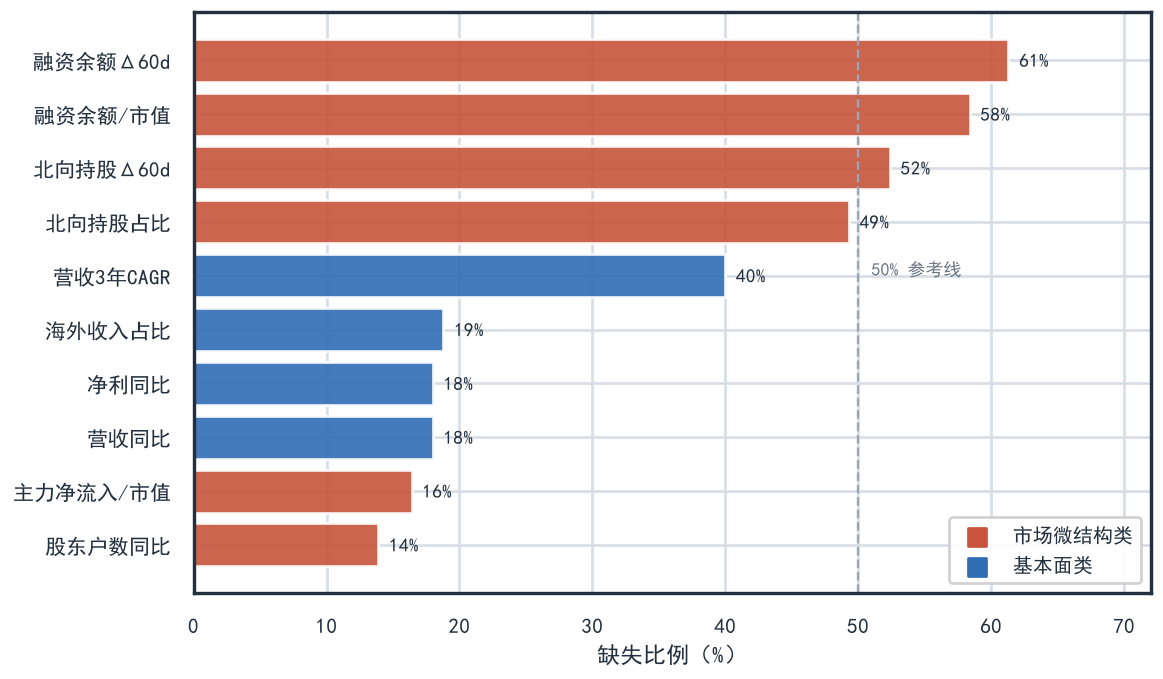
\includegraphics[width=\textwidth]{F5_特征缺失率.png}
\caption{各候选特征的缺失比例。红色为市场微结构类（融资余额、北向持股、主力净流入等），蓝色为基本面类。缺失最重的四个特征均为市场微结构类，缺失约 $49\%$ 至 $61\%$，远高于基本面类。}
\label{fig:missing}
\end{figure}

这一缺失并非随机：市场微结构数据仅覆盖沪深港通标的、融资融券标的，且自相应交易机制推出后才有记录，覆盖的公司—年份天然受限；若强行填补，将在近半数样本上引入大量人为构造值，污染信号。因此在特征选择阶段对缺失率过高（约超过一半）的市场微结构特征予以剔除，不纳入模型；基本面特征的少量缺失则以中位数填补，使模型建立在覆盖完整、口径一致的基本面信息之上。

本章诊断出的三类问题——强共线性、偏态与极端值、严重缺失——共同决定了后续处理流水线：以正则化与特征选择压缩冗余、以缩尾与树模型吸收偏态和离群值、以剔除高缺失特征保证口径一致。下一章先从特征工程的时点对齐与算术耦合审查入手。

\chapter{特征工程}\label{ch:feature}
特征工程的首要任务不是构造更多特征，而是保证每个特征都“干净”：既不含在使用时点尚不可得的信息，也不与目标共用构造分量。前者是\textbf{前视泄漏}（时间泄漏），后者是\textbf{算术耦合}（目标泄漏）。任一种泄漏都会让样本内表现虚高、样本外失效，并使归因失去意义。本章先依次封堵这两类泄漏，再交代标准化与趋势特征的构造。

\section{时点对齐：防前视泄漏}
财务数据存在公告滞后：某报告期的财报通常在期末之后 $1$ 至 $3$ 个月才公告。若把财务指标按\emph{报告期末}时点并入特征，就等于在公告日之前提前使用了尚未公开的信息——这是典型的前视泄漏，会让模型看似精准、实则不可复现。本研究采用时点对齐：每个特征在任一使用时点只取“当时最近一次已公告”的值，绝不使用公告日之后才可得的数据（图~\ref{fig:pit}）。市值、市销率、北向持股等市场类数据本身按日更新、无公告滞后，按交易日对齐。

\begin{figure}[htbp]
\centering
\begin{tikzpicture}[font=\sffamily, >={Stealth[length=2.6mm]}]
% —— 时间轴 ——
\draw[->, line width=1pt, color=ink] (0,0.5) -- (14,0.5);
\node[color=ink, font=\footnotesize] at (14,0.85){时间};
% 两个时点刻度
\draw[line width=1.4pt, brandred] (3,0.28) -- (3,0.72);
\draw[line width=1.4pt, brandblue] (8,0.28) -- (8,0.72);
\node[above=2pt, align=center, font=\small\bfseries, color=brandred] at (3,0.72){报告期末\\[-2pt]{\footnotesize\color{ink} 例：2023Q3 末}};
\node[above=2pt, align=center, font=\small\bfseries, color=brandblue] at (8,0.72){财报公告日\\[-2pt]{\footnotesize\color{ink} 期末后 1--3 个月}};
% —— 两段相位条 ——
\fill[brandred!12, rounded corners=2pt] (3,-0.35) rectangle (8,0.05);
\node[color=ink, font=\footnotesize] at (5.5,-0.15){滞后期 · 该期财务尚未公开};
\fill[brandgreen!18, rounded corners=2pt] (8,-0.35) rectangle (13.6,0.05);
\node[color=ink, font=\footnotesize] at (10.8,-0.15){已公告 · 可并入特征};
% —— 底部要点 ——
\node[anchor=west, color=brandred, font=\footnotesize] at (0.1,-0.95){\textbf{×}\, 若按报告期末并入财务 $\to$ 前视泄漏};
\node[anchor=west, color=brandgreen, font=\footnotesize] at (7.7,-0.95){\checkmark\, 本研究：自公告日起并入};
\end{tikzpicture}
\caption{时点对齐示意。财报在报告期末后 $1$ 至 $3$ 个月才公告；若在报告期末即并入该期财务（红）便使用了尚未公开的信息，构成前视泄漏。本研究只在公告日及之后（绿色区）使用该期财务，任一时点取当时最近一次已公告的值。}
\label{fig:pit}
\end{figure}

\section{算术耦合审查：防目标泄漏}
第二类泄漏更隐蔽：特征在\emph{公式}上与目标共用构造分量。目标 $Y$ 由 $\ln(\text{市值}/\text{营收})$ 剥离而来，任何在定义中含有营收或市值的特征，都会与 $Y$ 产生机械相关（伪相关），而非反映经济驱动。例如净利率 $=$ 净利$/$营收，其分母与 $Y$ 的分母同为营收，二者天然相关，但这种相关来自算术、并不表示“高净利率导致高估值”。

因此对全部 $42$ 个候选特征逐一审查其构造是否含营收或市值，并按类别汇总（图~\ref{fig:couple}）。结果显示：杠杆/流动性、海外两组完全无算术耦合，定义上与营收、市值均独立，是做较干净关联归因（乃至进一步因果性探讨）的必要前提；盈利能力、成长、费用/研发等组含较多与营收耦合的特征，所有权/情绪、市场流动性组则含与市值耦合的特征。这些耦合特征仍可进入模型用于关联性解释，但其系数不能被解读为因果。

\begin{figure}[htbp]
\centering
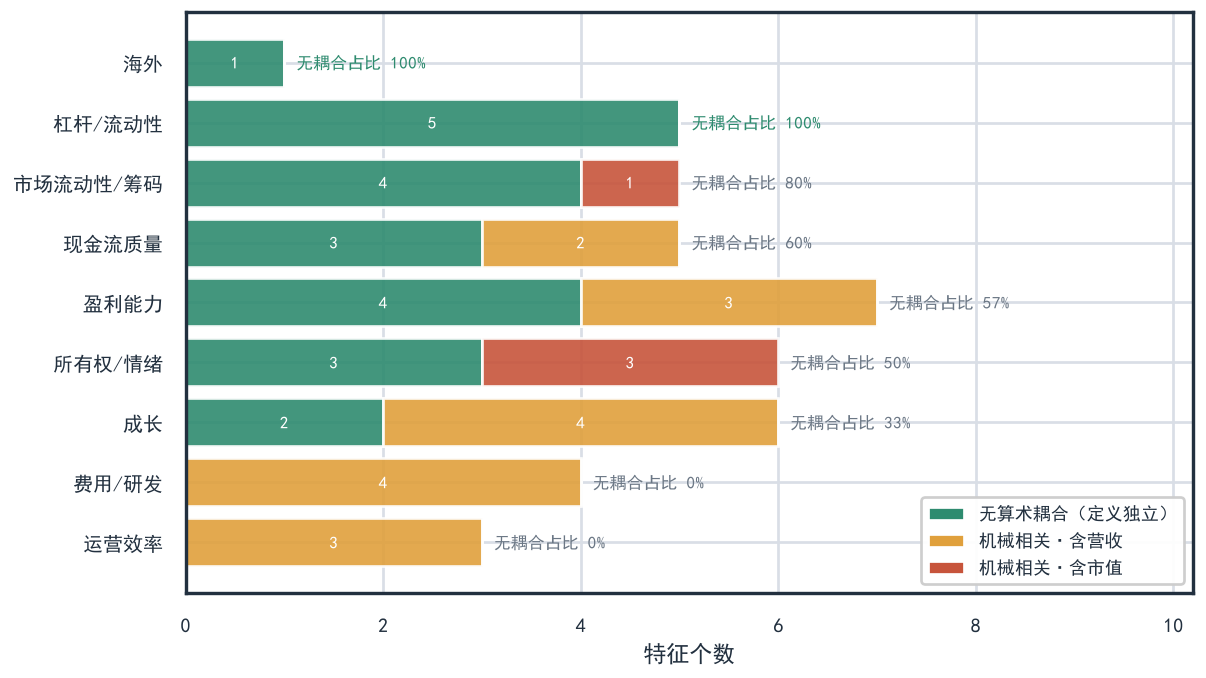
\includegraphics[width=\textwidth]{F8_算术耦合诊断.png}
\caption{各类特征与目标的算术耦合诊断。绿色为定义上与营收、市值均独立的无耦合特征，黄色为含营收、红色为含市值的机械相关特征；行尾为各组无耦合占比。杠杆/流动性（$5/5$）与海外（$1/1$）两组完全无耦合，是较干净关联归因的前提（仍非因果断言）。}
\label{fig:couple}
\end{figure}

这一区分是后续推断的基础：较干净的关联归因只建立在无耦合组之上；即便如此，本报告仍守在关联层、不作因果断言（详见稳健性与推断一章）。需强调，算术耦合刻画的是\emph{特征与目标}之间的关系，与第\ref{ch:eda}章的共线性（\emph{特征与特征}之间）是两个不同的问题：前者关乎归因是否为伪，后者关乎系数是否稳定。

\section{标准化与趋势特征}
最后是两点构造处理。其一，标准化：L1 选择与线性白盒模型对特征量纲敏感，故对其输入做 z 标准化（减均值、除标准差），使系数可比、正则化对各特征公平；梯度提升树基于取值排序分裂，不需标准化。其二，趋势特征：除水平值外，另构造毛利率、净利率的环比变化，作为“再定价触发”特征，以捕捉盈利能力边际改善或恶化对估值的影响。

至此，特征已完成防泄漏与构造，但 $42$ 个候选仍偏多、且如第\ref{ch:eda}章所示存在显著共线。下一章以 L1 正则化做特征选择，从中筛出稳定、互补的子集。

\chapter{特征选择}\label{ch:select}
经过第\ref{ch:feature}章的防泄漏处理，候选特征仍有 $42$ 个。直接把它们全部投入模型有两重风险，且均已在前文显现：其一，样本以公司为簇仅 $14$ 家、远少于特征数，灵活模型会过拟合（第\ref{ch:data}章）；其二，特征间高度共线，无约束系数在相关特征间任意分配、既不稳又可能符号反转（第\ref{ch:eda}章）。因此需要一道客观、可复现的特征选择，把候选压缩成一个既稳定又互补的子集：既保留解释力，又去掉冗余与噪声。本研究用 L1（Lasso）正则化完成这一步，其惩罚强度由按公司分组的交叉验证自动确定。

\section{L1 正则化}
L1 正则化在最小二乘损失上加一项与各系数绝对值之和成正比的惩罚，强度记为 $\alpha$。这一惩罚的特点是会把不重要特征的系数\emph{精确压到零}（而非仅仅缩小），因而天然兼具“收缩”与“选择”：$\alpha$ 越大，被保留的非零特征越少。问题于是归结为如何客观地选定 $\alpha$——太小会选入冗余、太大会丢掉有用信息。

\section{基于交叉验证的惩罚强度选定}
$\alpha$ 不能用拟合同一批数据的表现来定，否则它会被调成迎合这批样本的偶然结构。\textbf{交叉验证}的做法是把数据分成若干折：每次留出一折作验证、用其余折拟合，轮流让每一折都当一次验证集，再对各折的验证表现取平均；在候选 $\alpha$ 网格上选平均验证表现最优者。如此，$\alpha$ 的优劣始终在“未参与拟合”的数据上评判。

这里的关键是\textbf{必须按公司分组}。观测并不独立：同一家公司贡献数十个季度，彼此高度相关、共享该公司的估值水位。若按普通随机分折，同一公司的季度会同时落入拟合集与验证集——验证集里其实是模型“见过”的公司，它便能借助公司固有水位把验证表现抬高，这是一种泄漏，会让选出的 $\alpha$ 过于乐观。本研究改用\textbf{按公司分组的交叉验证}（GroupKFold）：把同一家公司的\emph{全部}观测整体分入同一折，使每个验证折只含模型完全没见过的公司。$14$ 家公司分为 $5$ 折、每折约 $3$ 家，$\alpha$ 因而是在“对全新公司外推”的标准下选定，与本报告“解释一家公司估值”的真实任务一致。

整个过程由程序在固定随机种子下自动完成：标准化输入、沿 $\alpha$ 网格做分组交叉验证、取最优 $\alpha$、保留系数非零的特征——无任何人工挑选，同一份代码可复现完全相同的 $17$ 个入选特征。这套按公司分组的交叉验证，也是后续超参数调优与留一家外推验证两章的共同基础。

图~\ref{fig:cv} 给出这一选择的实际结果：验证误差随 $\alpha$ 呈 U 形——$\alpha$ 过小则特征过多、过拟合，$\alpha$ 过大则欠拟合——在 $\alpha\approx0.026$ 处最低，据此自动选定，对应保留 $17$ 个特征。需说明，此处验证误差取自留公司外推的\emph{线性选择模型}，仅用于客观定位 $\alpha$；最终模型在更强方法下的解释力（留一家 $R^2\approx0.45$）另见模型验证一章。

\begin{figure}[htbp]
\centering
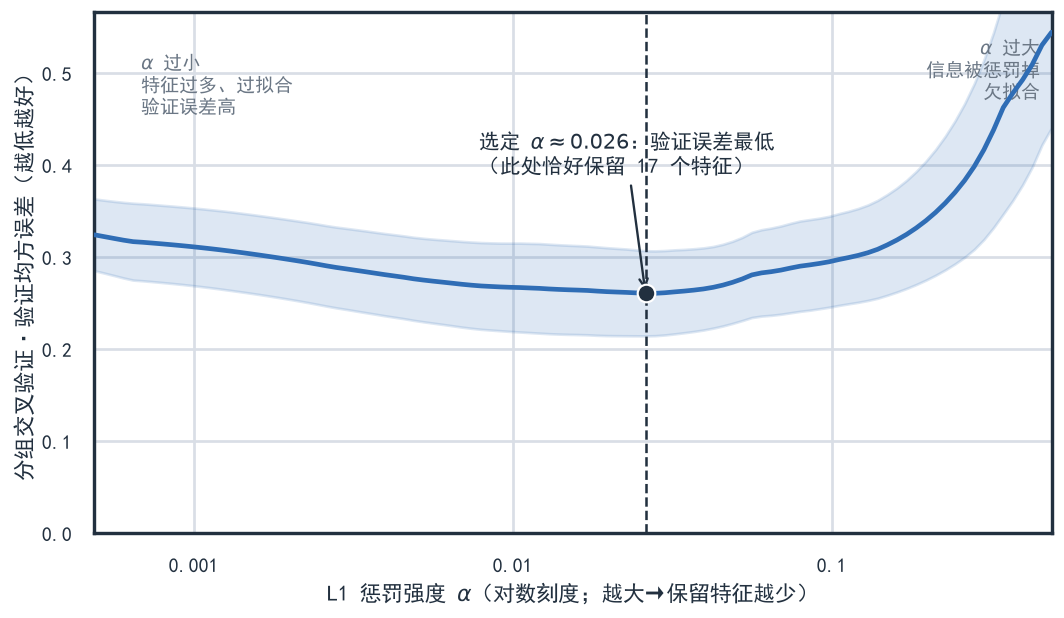
\includegraphics[width=0.85\textwidth]{F_CV选择.png}
\caption{按公司分组交叉验证选定 L1 惩罚强度 $\alpha$。蓝线为分组交叉验证的验证均方误差（越低越好），阴影为跨折 $\pm1$ 标准误。曲线呈 U 形：$\alpha$ 过小则特征过多、过拟合，$\alpha$ 过大则欠拟合；误差在 $\alpha\approx0.026$ 处最低（竖虚线），据此自动选定，此时恰保留 $17$ 个特征。该验证误差来自留公司外推的线性选择模型，仅用于定位 $\alpha$。}
\label{fig:cv}
\end{figure}

\section{特征选择结果}
在选定的 $\alpha$ 下，L1 把 $42$ 个候选压缩为 $17$ 个、剔除 $25$ 个。每个被删特征都可按它与最相关保留特征的相关系数 $r$ 审视剔除是否合理（逐特征明细见附录~\ref{app:l1}）：$15$ 个属\textbf{高共线冗余}（$r\geq0.5$），其信息已被某保留特征覆盖，例如现金比率与速动比率相关 $0.98$、流动比率与速动比率 $0.90$，同组保留其一即可；$10$ 个属\textbf{弱信号}（$r<0.5$），与目标关联微弱、被惩罚归零。两类均不携带保留集以外的独立信息。

最终保留的 $17$ 个特征横跨盈利、成长、运营效率、杠杆与流动性、研发与市场结构等互补维度（各特征定义见附录~\ref{app:datadict}），彼此冗余度低，构成后续建模的输入。下一章即在其上构建模型，并解读系数方向。

\chapter{建模}\label{ch:model}
经过前几章，已得到一个口径干净、防泄漏、并经 L1 压缩为 $17$ 个互补特征的建模数据。本章在其上建立模型，并先确立一条贯穿全报告的定位：在这一样本规模下，机器学习模型只承担\emph{描述}，不承担\emph{推断}。

\section{建模定位：机器学习的描述性角色}
样本只有 $14$ 家公司，而识别各驱动系数所依赖的\emph{有效独立簇}比 $14$ 还少（约 $5$ 个，详见稳健性与推断一章）。在这种规模下，任何灵活的机器学习模型——无论如何调参——对未见过公司的外推都很脆弱，单个特征的重要性与系数都带有很大的抽样方差（这一点将由后文的自助稳定性区间量化）。因此本报告\textbf{不让机器学习承担可信推断}：真正的系数推断与因果性探讨交给面板/公司内回归配合少簇稳健方法（详见稳健性与推断一章）；本章与可解释性一章的机器学习模型只作\textbf{描述性归因}——给出“哪些指标与超额估值同向、量级大致如何”的一张地图，而非可信赖的点估计。

这一定位决定了建模取向：以强约束、低复杂度换取稳健与可解释，而不是追逐样本内拟合。具体复杂度上限与调参见下一章。

\section{两个互补的描述模型}
本章建立两个模型，互为印证。

\textbf{其一，浅树梯度提升树}（描述主模型）。深度受限——叶数与树深均压在很低的档位（针对 $14$ 簇\emph{先验}设定，见下一章），以防过拟合。约束\textbf{最小化}：只对资产负债率施加“杠杆越高、估值越低”的单调方向约束——这是唯一在经济上方向无歧义、且经独立三角验证（见稳健性与推断一章的 H2）的方向；其余特征一律不约束，由数据决定方向与符号。树的预测落在训练样本的取值域内、天然有界，对新公司外推稳健，留一家外推 $R^2\approx0.45$。形式上，它是 $M$ 棵浅树的加法集成
\[
  \widehat{Y}(x)\;=\;\sum_{m=1}^{M}\eta\,h_m(x),
\]
每棵 $h_m$ 为叶数 $\leq 7$、深度 $\leq 3$ 的回归树，$\eta$ 为学习率，逐棵拟合上一轮的残差（故称“提升”）；最终 $M=200$、$\eta=0.05$（见下一章表~\ref{tab:hp}）。

\textbf{其二，白盒线性模型}（ElasticNet）。它完全透明、系数可手算，作为\emph{样本内}的可解释对照，给出每个特征的方向与量级。两个模型分工互补：梯度提升树的预测落在训练样本的取值域内、有界且对离群值稳健，故承担对新公司的外推；白盒线性模型完全透明，承担样本内的方向解读。二者方向一致时，结论更可信。

\section{入选特征的系数方向}
图~\ref{fig:coef} 给出白盒线性模型对 $17$ 个入选特征的标准化系数（按大小排序，绿色为正向、红色为负向）。可读出几条方向：

\begin{itemize}
  \item \textbf{杠杆最强且为负}：资产负债率 $-0.26$——低杠杆对应高估值。
  \item \textbf{成长为负}：营收 $3$ 年复合增速 $-0.08$、营收同比 $-0.04$——成长越高，超额估值反而越低。这与“成长享溢价”的通常直觉相反，是本研究样本的特征，后文称之为\emph{成长折价}。
  \item \textbf{盈利为正}：净利率 $+0.13$——高利润率对应溢价。
  \item 市场结构类（振幅、Amihud 非流动性、融资余额占市值等）量级中等，属关联层，其中含市值成分者尤须谨慎（见第\ref{ch:feature}章的算术耦合审查）。
\end{itemize}

\begin{figure}[htbp]
\centering
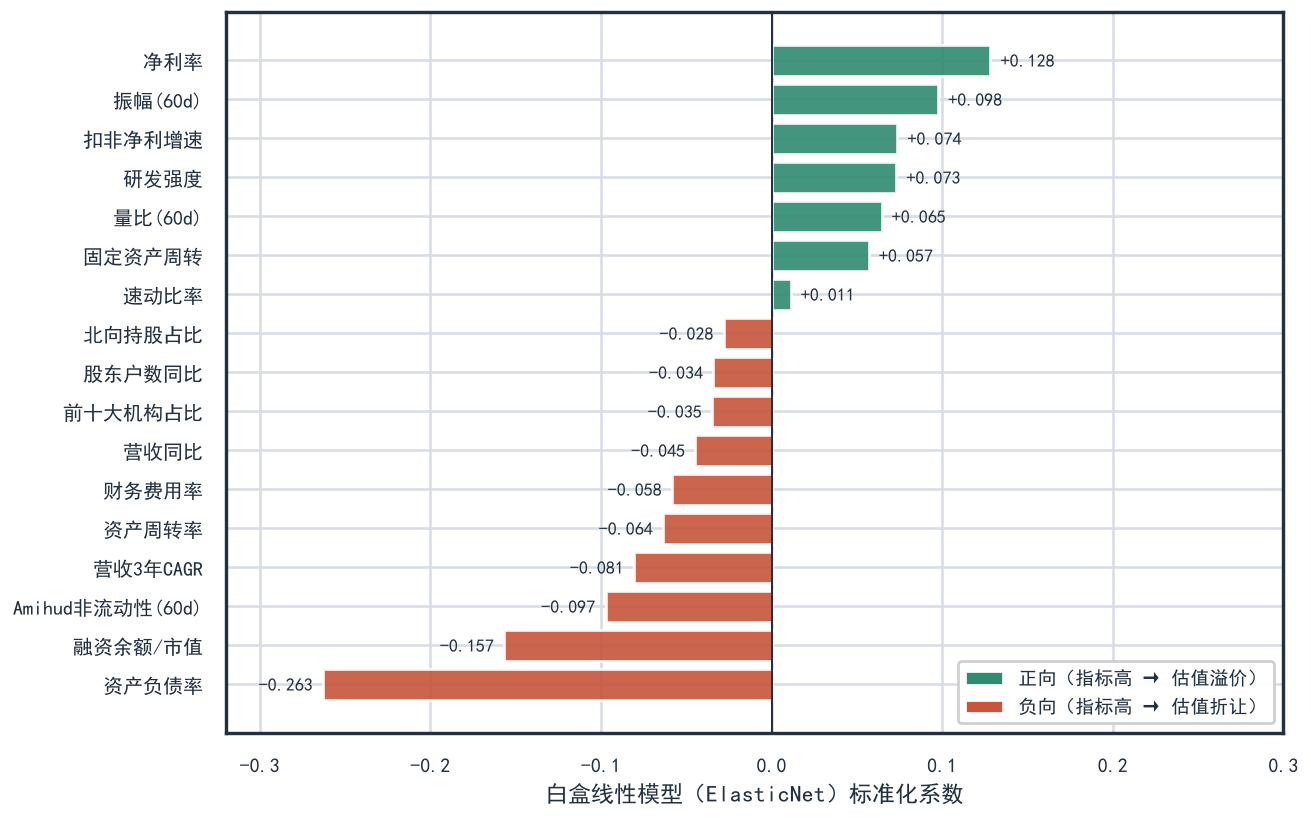
\includegraphics[width=0.92\textwidth]{F10_入选特征系数.png}
\caption{白盒线性模型（ElasticNet）对 $17$ 个入选特征的标准化系数。绿色为正向（指标越高、估值越偏溢价），红色为负向（指标越高、估值越偏折让）。资产负债率最负（$-0.26$，低杠杆对应高估值），营收 $3$ 年复合增速为负（$-0.08$，成长折价），净利率最正（$+0.13$）。}
\label{fig:coef}
\end{figure}

白盒模型完全透明、可写成显式表达式：对 $z$ 标准化后的 $17$ 个特征，超额估值的线性预测为
\[
  \widehat{Y}\;=\;\sum_{j=1}^{17}\beta_j\,z(x_j),
\]
目标与各输入均已中心化，故截距约为零；标准化系数 $\beta_j$ 列于表~\ref{tab:encoef}，可直接读出各特征的方向与相对量级。

\begin{table}[htbp]
\caption{白盒线性模型（ElasticNet）的 $17$ 个标准化系数 $\beta_j$（按绝对值降序）。正值表示该指标越高、估值越偏溢价，负值反之。}
\label{tab:encoef}
\footnotesize
\renewcommand{\arraystretch}{1.3}
\begin{tabular*}{\textwidth}{@{\extracolsep{\fill}}lr lr lr@{}}
\toprule
\textbf{\color{brandblue}特征} & \textbf{\color{brandblue}$\beta$} & \textbf{\color{brandblue}特征} & \textbf{\color{brandblue}$\beta$} & \textbf{\color{brandblue}特征} & \textbf{\color{brandblue}$\beta$} \\
\midrule
资产负债率 & $-0.26$ & 扣非净利增速 & $+0.07$ & 营收同比 & $-0.04$ \\
融资余额/市值 & $-0.16$ & 研发强度 & $+0.07$ & 前十大机构占比 & $-0.03$ \\
净利率 & $+0.13$ & 量比(60d) & $+0.06$ & 股东户数同比 & $-0.03$ \\
振幅(60d) & $+0.10$ & 资产周转率 & $-0.06$ & 北向持股占比 & $-0.03$ \\
Amihud非流动性(60d) & $-0.10$ & 财务费用率 & $-0.06$ & 速动比率 & $+0.01$ \\
营收3年CAGR & $-0.08$ & 固定资产周转 & $+0.06$ & & \\
\bottomrule
\end{tabular*}
\end{table}

这些是\textbf{描述性}系数。在特征间存在共线的情形下（见第\ref{ch:eda}章），单个特征的系数会在相关特征之间分配，因此\textbf{这些系数是关联层的方向描述、而非精确的因果效应}。每个方向\emph{有多稳}、\emph{是否可信}，分别由可解释性一章的自助稳定性区间、与稳健性与推断一章的少簇稳健推断回答。本章只给出方向的地图，可信度的裁定留给后两章。

\chapter{超参数与交叉验证}\label{ch:cv}
模型的复杂度（树有多深）与泛化能力如何评估，是小样本下最易高估解释力的两处。本章交代复杂度上限如何确定、以及如何在不泄漏的前提下衡量外推能力。

\section{复杂度上限与浅树设定}
在 $14$ 家公司的规模下，模型复杂度必须\emph{事先}压低。图~\ref{fig:lc} 的学习曲线给出实证：随训练样本量增加，训练集 $R^2$ 稳定在约 $0.85$，而分组交叉验证 $R^2$ 只有约 $0.45$；二者之差（过拟合间隙）很大，且不随样本量增加而收窄——本研究的样本本就只有 $14$ 家公司，无法通过扩大样本量来缩小。这说明灵活模型在样本内能拟合得很好，但对全新公司的外推被限制在约 $0.45$。

\begin{figure}[htbp]
\centering
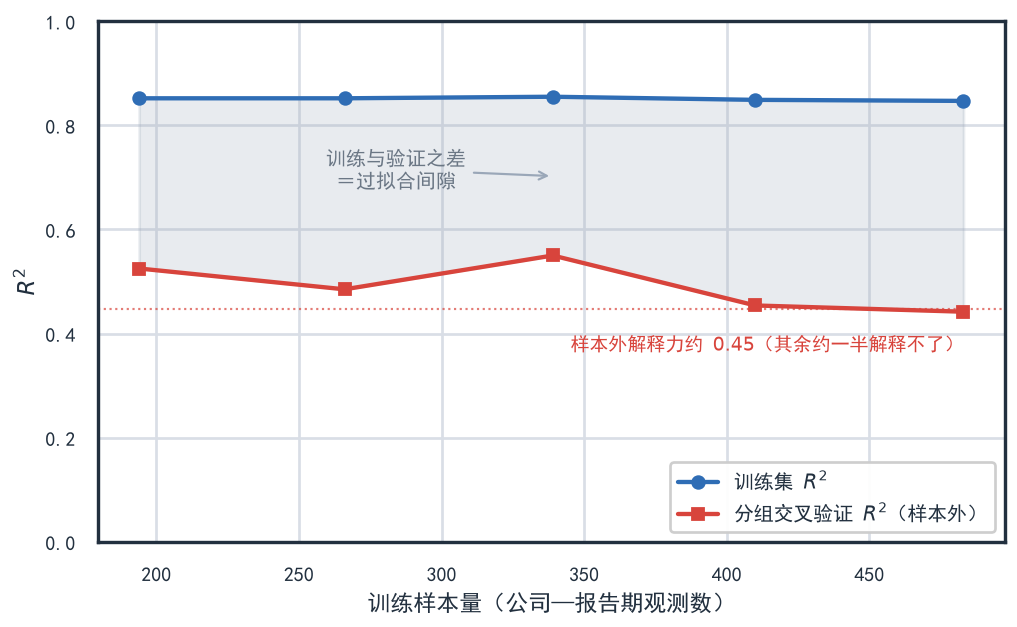
\includegraphics[width=0.86\textwidth]{F_学习曲线.png}
\caption{学习曲线：训练集 $R^2$ 与分组交叉验证 $R^2$ 随训练样本量的变化。训练 $R^2$ 稳定在约 $0.85$，分组交叉验证 $R^2$ 约 $0.45$；二者之差为过拟合间隙，不随样本量收窄（样本仅 $14$ 家公司）。虚线为样本外解释力的大致水平。}
\label{fig:lc}
\end{figure}

因此把树的复杂度\emph{先验地}压在很浅的档位（叶数不超过 $7$、树深不超过 $3$）：这一上限按“有效样本仅约十余家公司、远少于特征数”的规模设定，而非看验证结果反复挑选。作为对照，放开复杂度上限时，自动调参会选出更深的树——样本内 $R^2$ 随之更高（过拟合更重），但对留出公司的外推不升反降。这从反面印证了浅树档位的必要。

用偏差—方差的语言可概括这一取舍：浅树偏差略高、方差低，深树则偏差低、方差高；在 $14$ 簇这样由方差主导的小样本里，方差为误差的主导来源，故宁可承受一点偏差以换取低方差——浅树正落在这一权衡的合理区间，也即学习曲线上训练与验证之差不再因加深模型而改善的位置。

\section{超参数与最优复杂度区间}
浅树并非主观设定，而是在一个预设的超参数网格上、由机器按分组交叉验证自动选出。可调超参数包括树的复杂度（叶数、树深）、学习率、正则化强度与采样比例等；其中树复杂度按前述先验封在浅档（叶数不超过 $7$、树深不超过 $3$），其余由搜索决定。最终选定的主要超参数见表~\ref{tab:hp}。

\begin{table}[htbp]
\caption{机器自动选定的主要超参数（按公司分组交叉验证搜索，固定随机种子）}
\label{tab:hp}
\renewcommand{\arraystretch}{1.25}
\begin{tabular*}{\textwidth}{@{\extracolsep{\fill}} l c l c l c @{}}
\toprule
\textbf{\color{brandblue}超参数} & \textbf{\color{brandblue}值} & \textbf{\color{brandblue}超参数} & \textbf{\color{brandblue}值} & \textbf{\color{brandblue}超参数} & \textbf{\color{brandblue}值} \\
\midrule
叶节点数 & $4$ & 学习率 & $0.05$ & L2 正则 & $1$ \\
最大树深 & $2$ & 树的棵数 & $200$ & L1 正则 & $2$ \\
最小叶样本 & $20$ & 行采样比例 & $0.6$ & 列采样比例 & $1.0$ \\
\bottomrule
\end{tabular*}
\end{table}

复杂度的取舍可由图~\ref{fig:sweet} 直观看到：随叶数增加，样本内 $R^2$ 单调上升（拟合越来越好），而分组交叉验证 $R^2$ 在约 $4$ 叶处见顶（约 $0.45$）后回落——这就是偏差-方差的最优区间。叶数过少则欠拟合、过多则过拟合（样本内升、外推降），最优复杂度恰落在浅档，与先验设定一致。

\begin{figure}[htbp]
\centering
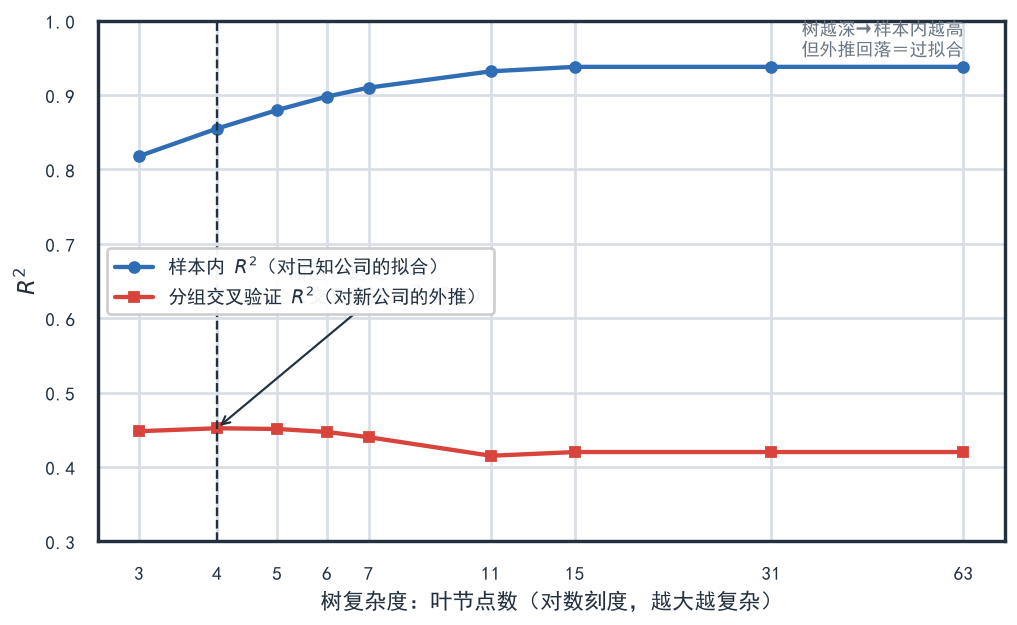
\includegraphics[width=0.70\textwidth]{F_甜区.png}
\caption{偏差-方差最优区间。横轴为树复杂度（叶节点数，对数刻度）。样本内 $R^2$ 随复杂度单调上升，分组交叉验证 $R^2$ 在约 $4$ 叶处见顶后回落；二者之差随复杂度加深而扩大（过拟合）。竖虚线为选定的 $4$ 叶。}
\label{fig:sweet}
\end{figure}

\section{嵌套交叉验证}
要报告\emph{无泄漏}的外推解释力，仅把特征选择放进折内还不够——连超参数调优也必须在折内完成，否则用全样本调出的超参再去“验证”留出的公司，仍是一处轻微泄漏。为此本研究采用\textbf{嵌套交叉验证}（图~\ref{fig:nested}）：外层留一家公司，内层仅在训练的其余 $13$ 家上重新完成缩尾、特征选择与调参，训练后才预测留出的那一家；留出公司全程不参与任何拟合步骤。

\begin{figure}[htbp]
\centering
\begin{tikzpicture}[font=\sffamily, >={Stealth[length=2.6mm]}]
\node[font=\small\bfseries, color=ink] at (0,3.25) {外层：留一家公司外推（$14$ 家轮流留出，共 $14$ 折）};
\node[draw=brandblue, line width=1pt, rounded corners=4pt, fill=brandblue!6, align=left,
      inner sep=9pt, font=\small, text width=7.3cm] (tr) at (-3.5,1.1)
  {\textbf{训练：其余 $13$ 家公司}\\[3pt] ① 分位缩尾 \,$\to$\, ② L1 特征选择\\[2pt] ③ 内层分组交叉验证选超参\\[2pt] ④ 拟合浅树 GBT};
\node[draw=brandred, line width=1pt, rounded corners=4pt, fill=brandred!6, align=center,
      inner sep=9pt, font=\small, text width=3.0cm] (te) at (4.1,1.1)
  {\textbf{留出：$1$ 家}\\[3pt]{\footnotesize 全程不参与训练}};
\draw[->, line width=1pt, color=ink] (tr) -- node[above, font=\footnotesize]{训好后预测} (te);
\node[align=center, font=\footnotesize, color=ink] at (0,-0.9)
  {汇总 $14$ 折的留出预测 \,$\Rightarrow$\, 留一家 $R^2$（无泄漏）};
\end{tikzpicture}
\caption{嵌套交叉验证示意。外层留一家公司；每个外折内部，缩尾、特征选择与超参数调优全部仅在训练的 $13$ 家上完成（①--④），训练后才预测留出的那家（⑤）。留出公司全程不参与拟合，故所得留一家 $R^2$ 无泄漏。}
\label{fig:nested}
\end{figure}

结果表明这处泄漏可忽略：嵌套的留一家 $R^2$ 为 $0.452$，与非嵌套的 $0.454$ 几乎相同；嵌套的留时段 $R^2$ 为 $0.455$。换言之，此前报告的留一家解释力本就是干净的。

\section{样本内与样本外：交叉对照}
对模型的解释力，本报告并报样本内与样本外两个口径，并明确各自含义，而非只取其一。
\begin{itemize}
  \item \textbf{样本内 $R^2$（约 $0.85$）}衡量模型对\emph{已见过的公司}拟合得多好。它是\emph{过拟合的诊断}、而非性能——小样本下灵活模型总能把已知数据拟合得很高，这个数字本身不说明泛化能力。
  \item \textbf{样本外 $R^2$（约 $0.45$）}衡量模型对\emph{从未见过的公司}外推得多好。这才是本报告采用的\emph{性能口径}。
\end{itemize}
二者之差（约 $0.40$）即过拟合的幅度，反映小样本下不可避免的方差。因此本报告以样本外为性能标准、样本内仅作诊断，两个口径透明并列、互相参照，不以样本内充当成绩。各级口径由“拟合”到“真外推”的逐层落差见图~\ref{fig:ladder}：样本内 $R^2$ 约 $0.85$，到分组交叉验证（留出公司）落到约 $0.44$，留时段外推 $0.50$、留一家外推 $0.45$；最大落差发生在样本内到样本外之间，几种样本外口径则彼此接近、稳定在约 $0.45$（对应误差见表~\ref{tab:metrics}）。

\begin{figure}[htbp]
\centering
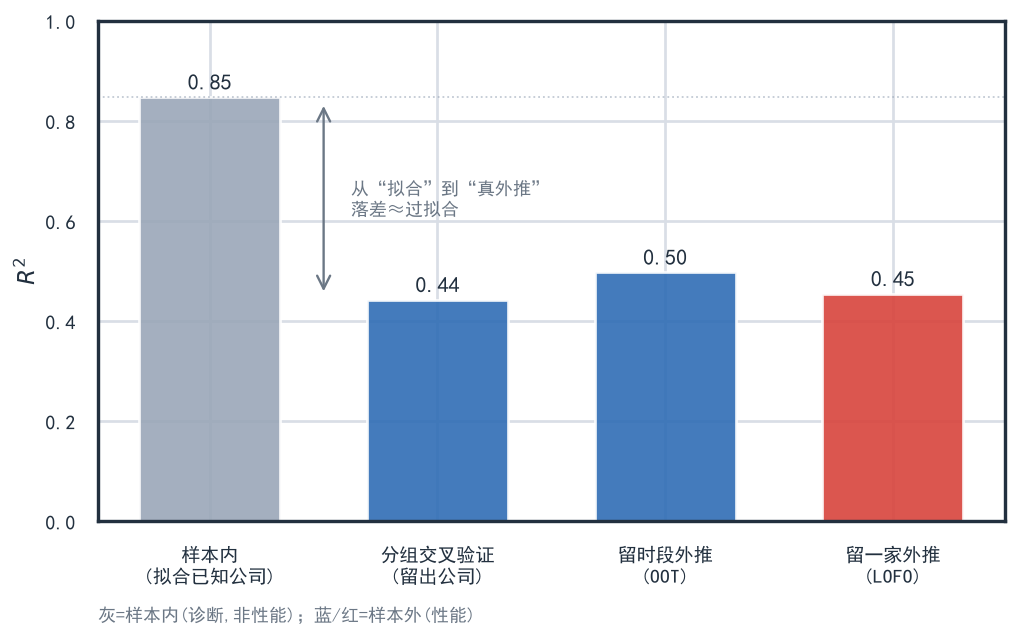
\includegraphics[width=0.82\textwidth]{F_R2阶梯.png}
\caption{解释力阶梯。灰柱为样本内（拟合已知公司，属诊断、非性能），蓝/红柱为样本外（对留出公司/时段的外推，属性能）。从样本内到样本外的落差即过拟合幅度；几种样本外口径稳定在约 $0.45$。}
\label{fig:ladder}
\end{figure}

\begin{table}[htbp]
\caption{各验证口径的解释力与误差}
\label{tab:metrics}
\renewcommand{\arraystretch}{1.25}
\begin{tabular*}{\textwidth}{@{\extracolsep{\fill}} l c c c @{}}
\toprule
\textbf{\color{brandblue}口径} & \textbf{\color{brandblue}$R^2$} & \textbf{\color{brandblue}均方根误差} & \textbf{\color{brandblue}平均绝对误差} \\
\midrule
样本内（拟合，诊断用） & $0.85$ & $0.27$ & $0.21$ \\
留时段外推（OOT） & $0.50$ & $0.53$ & $0.43$ \\
留一家外推（LOFO） & $0.45$ & $0.50$ & $0.41$ \\
\bottomrule
\end{tabular*}
\end{table}

\chapter{模型验证}\label{ch:validation}
本章的结论可概括为一句：\textbf{基本面只能解释新公司估值差异的一半；另一半是情绪与公司特异因素，而非模型本身的缺陷。}下面分三步说明——模型确实能外推（那一半是真的）、另一半是什么、以及这“一半”本身也带不确定性。

\section{留一家外推验证}
要确认那约 $0.45$ 的解释力是真实的外推能力、而非样本内的过拟合假象，须看模型对\emph{从未参与训练}的公司预测得如何。图~\ref{fig:predact} 把每个“公司—报告期”的留一家外推预测与真实超额估值逐点对照：点云整体沿上升趋势分布（蓝线），说明模型抓住了跨公司估值差异的\emph{方向}与大致幅度；但散布明显、趋势线比完美预测线平缓，说明它只能解释约一半、无法精确复现。研究主体移为通信（红点）集中在右上的溢价区，其溢价被模型部分、而非全部预测到。这一外推已在前一章经嵌套交叉验证确认无泄漏，故 $R^2\approx0.45$ 是干净的真外推解释力。

\begin{figure}[htbp]
\centering
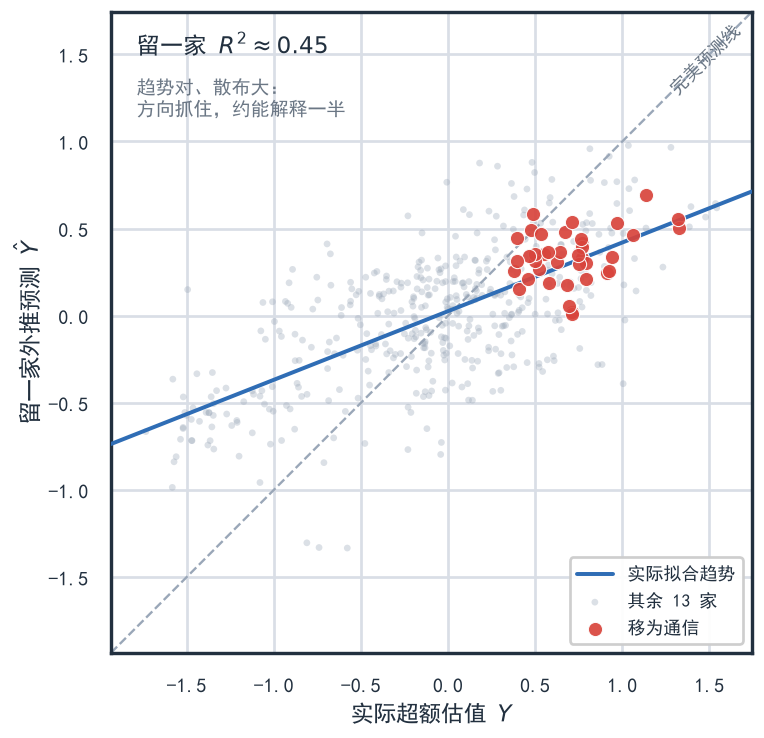
\includegraphics[width=0.62\textwidth]{F_预测实际.png}
\caption{留一家外推的预测与实际。每点为一个公司—报告期，横轴为真实超额估值、纵轴为留出该公司后对其的外推预测；灰虚线为完美预测线，蓝线为实际拟合趋势。趋势对、散布大，对应 $R^2\approx0.45$；移为通信（红）集中于溢价区。}
\label{fig:predact}
\end{figure}

\section{特征组的增量贡献}
哪些特征承载了这约 $0.45$ 的样本外解释力？逐步加入特征组并重估留一家 $R^2$（图~\ref{fig:abl}）：仅资产负债率一项即达约 $0.48$，其后加入成长、盈利与质量、市场结构各组，$R^2$ 几乎走平。按公司整块重抽得到的 $90\%$ 区间很宽（约 $0.2$--$0.6$），各步点估计都落在彼此区间之内——故不能认定某一组带来了\emph{显著}的样本外增益。可稳妥得出的是量级结论：跨公司可外推的估值差异\textbf{主要由杠杆承载}，其余特征组的增量贡献落在小样本噪声之内。这与杠杆为最强稳健驱动一致，也再次说明机器学习在此的价值在于“用了哪些特征”的描述，而非复杂模型的预测增益。

\begin{figure}[htbp]
\centering
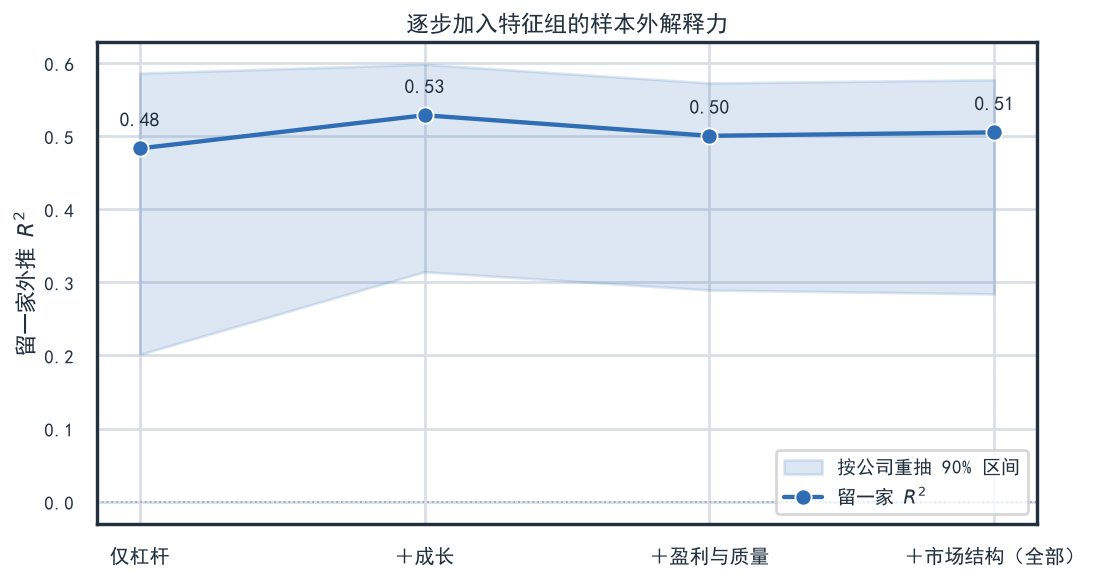
\includegraphics[width=0.80\textwidth]{F_消融.png}
\caption{逐步加入特征组的留一家外推 $R^2$。点为 $R^2$ 点估计，阴影为按公司整块重抽的 $90\%$ 区间。仅杠杆即达约 $0.48$，其后各组几乎走平、且点估计均落在彼此的宽区间内，说明杠杆以外特征组的样本外增量贡献在小样本噪声之内。}
\label{fig:abl}
\end{figure}

\section{残差诊断}
留一家残差（实际超额估值减外推预测）可进一步暴露模型行为（图~\ref{fig:resid}）。残差对拟合值无明显结构、整体均值近零，说明模型没有系统性的高估或低估倾向。但逐家来看，个别公司存在系统性偏移：移为通信的残差中位为正（模型对其\emph{低估}），日海智能、利尔达等为负。这些公司层面的固定偏移，正是基本面解释不了、与公司绑定的特异成分——也即下一节“情绪缺口”在残差上的直接体现。

\begin{figure}[htbp]
\centering
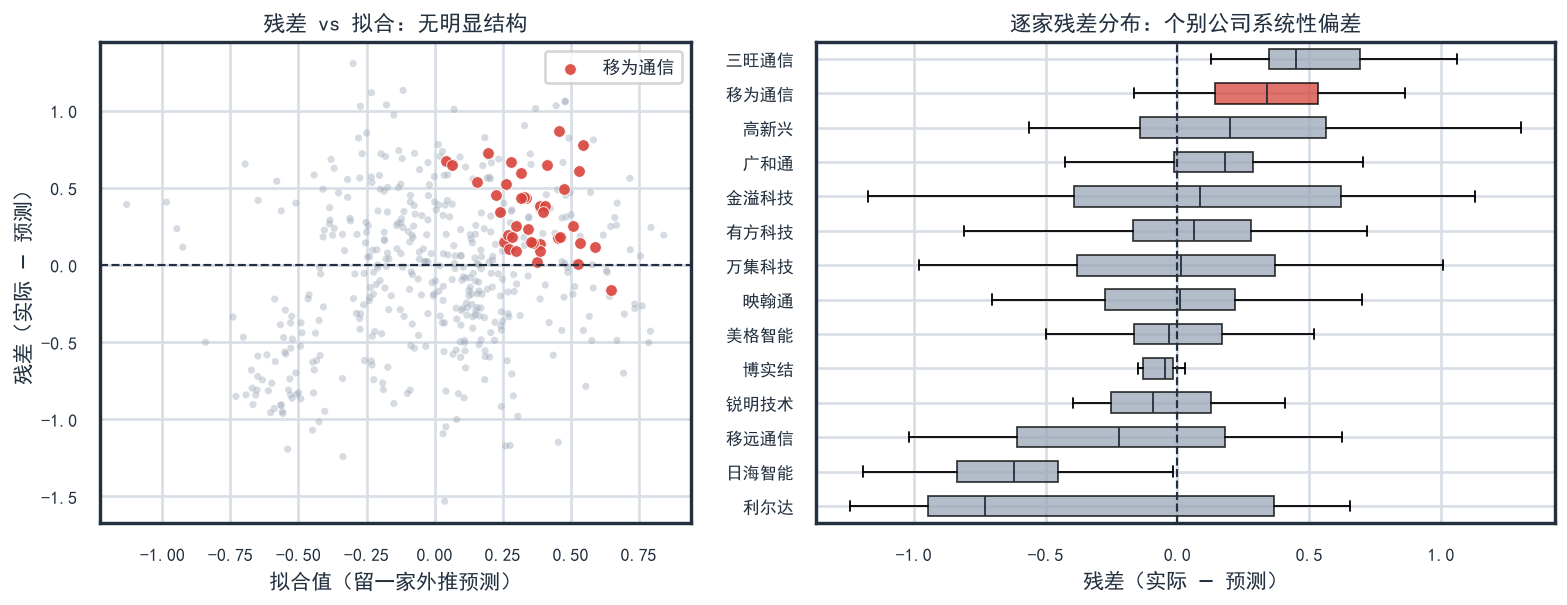
\includegraphics[width=\textwidth]{F_残差诊断.png}
\caption{留一家外推的残差诊断。左：残差对拟合值无明显结构、均值近零；右：逐家残差分布，个别公司存在系统性偏移（移为通信中位为正、模型对其低估），即基本面解释不了的公司特异成分。}
\label{fig:resid}
\end{figure}

\section{未解释部分的来源}
未解释的约一半\emph{不是}模型调参不当，而是与基本面正交的成分——市场情绪、叙事、错误定价及小样本噪声。两条佐证。其一，把“基本面应得的估值”（用其余 $13$ 家的定价规律外推、不含该公司自身）与实际估值比较，可按溢价/折让对全样本做错误定价筛查，留一家外推下判别 AUC 约 $0.81$（小样本下方差较大，用于方向性筛查）。其二，移为通信的溢价分解最为直观（图~\ref{fig:decomp}）：其实际超额估值 $+0.70$ 中，基本面可解释的约 $+0.34$（主要来自低杠杆，占 $49\%$），其余约 $+0.36$（占 $51\%$）属基本面解释不了的“情绪缺口”——几乎各占一半。后者更易随市场预期回摆。

\begin{figure}[htbp]
\centering
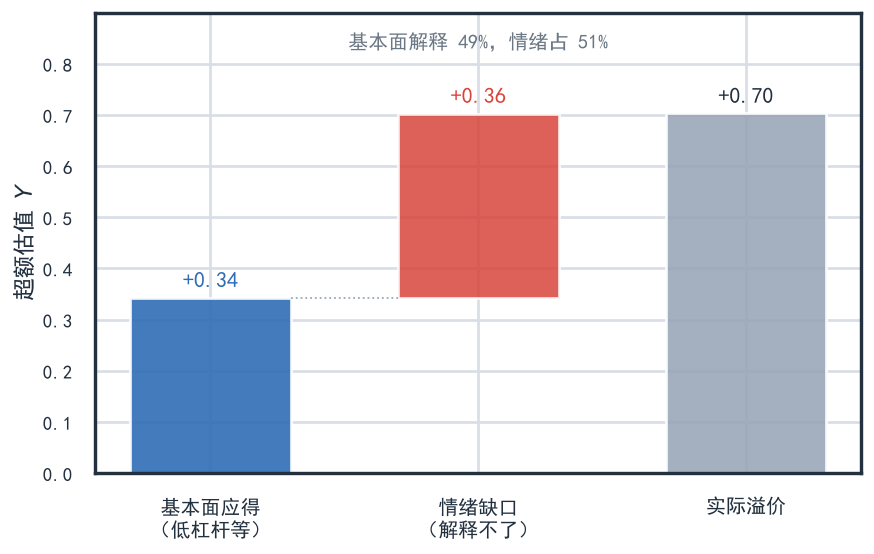
\includegraphics[width=0.66\textwidth]{F_移为分解.png}
\caption{移为通信溢价分解。实际超额估值 $+0.70$ 拆为基本面应得（$+0.34$，主要为低杠杆）与情绪缺口（$+0.36$，基本面解释不了）两部分，约各占一半。基本面应得由其余 $13$ 家的定价规律外推得到，不含移为自身。}
\label{fig:decomp}
\end{figure}

\section{样本外解释力的不确定性}
这约 $0.45$ 是一个量级、而非精确值。目标 $Y$ 取自第一阶段回归的残差（属估计量、非直接观测），且真正独立的有效簇只有约 $5$ 个（详见稳健性与推断一章）；因此报告中一律以“基本面解释了大约一半”来表述。

\chapter{可解释性}\label{ch:interp}
本章打开模型，看它把估值差异归到了哪些特征上。这是一张\textbf{描述性的地图}——它回答“模型用了哪些指标、量级大致如何”，方向是否经得起严格检验则交由下一章。

\section{SHAP 重要性与稳定性}
SHAP 把模型对每个样本点的预测按 Shapley 值精确分解为各特征的可加贡献
\[
  \widehat{Y}(x)\;=\;\phi_0+\sum_{j=1}^{17}\phi_j(x),\qquad \phi_0=\mathbb{E}\big[\widehat{Y}\big],
\]
其中 $\phi_j(x)$ 为特征 $j$ 在该点的贡献、$\phi_0$ 为全样本基准；对全样本取 $|\phi_j|$ 的均值即该特征的整体重要性。配合按公司成对聚类自助（重抽 $14$ 家公司、整条管线重拟合 $400$ 次），每个特征的重要性都带上区间与“被选中频率”，结果见图~\ref{fig:shap}。

\begin{figure}[htbp]
\centering
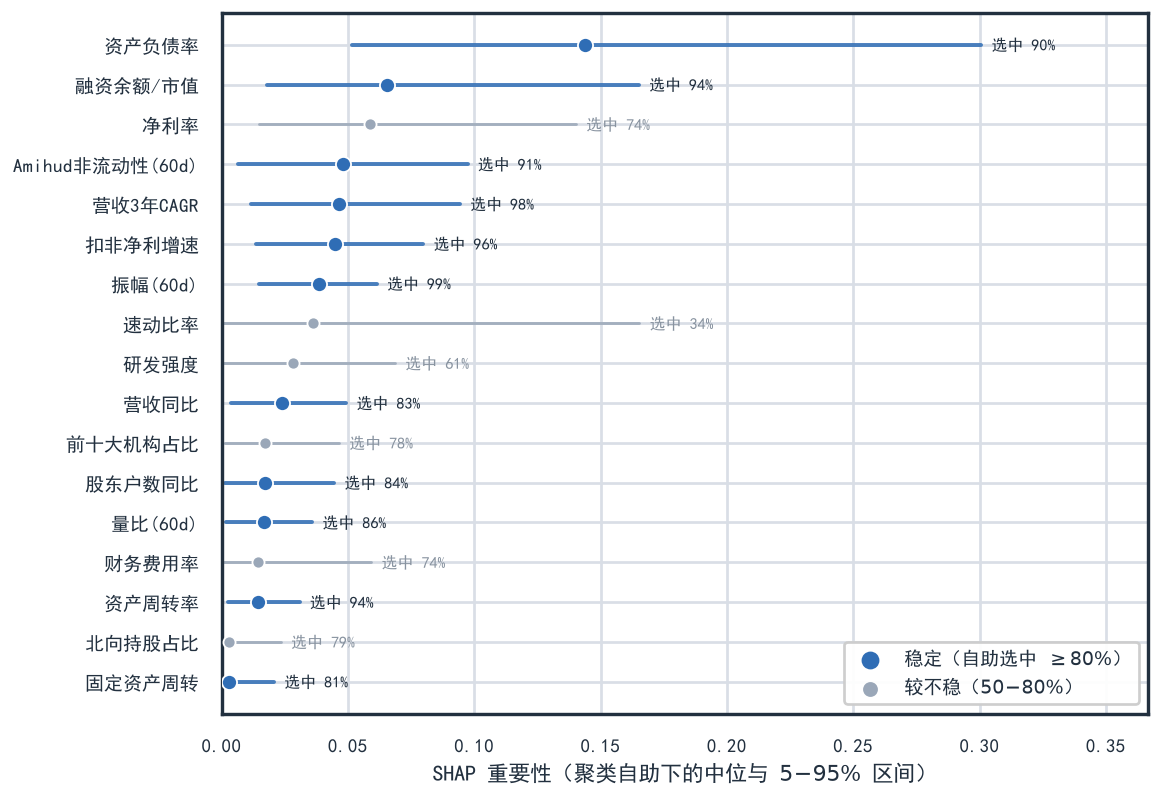
\includegraphics[width=\textwidth]{F_SHAP稳定性.png}
\caption{入选特征的 SHAP 重要性及其聚类自助稳定性。圆点为自助中位重要性，横线为 $5\!-\!95\%$ 区间，行尾为该特征在自助中被选中的频率；蓝色为稳定特征（选中 $\geq80\%$），灰色为较不稳（$50\!-\!80\%$）。}
\label{fig:shap}
\end{figure}

重要性的排序由资产负债率（杠杆）领衔，其后是融资余额占市值、净利率，以及若干成长与市场结构特征。更有用的是稳定性的分层：杠杆、成长（营收复合增速、扣非净利增速）与几个市场结构特征构成一个\textbf{稳定核心}——它们在自助中几乎每次入选、重要性区间不贴零；而盈利类特征（净利率、毛利率）的被选中频率不足 $80\%$，其入选与重要性都随样本而变。换言之，可放心解读的是这个核心，而非完整的 $17$ 项排序。

\section{驱动的函数形状}
SHAP 给出方向与量级，部分依赖（partial dependence）进一步给出\emph{形状}：固定其余特征、令目标特征在其取值域内变化，模型预测的平均响应即该特征的边际形状（图~\ref{fig:pdp}）。三个核心特征形状各异：资产负债率呈单调陡降（含单调约束），落差集中在负债率约 $20\%$--$65\%$ 区间；营收复合增速呈单调递减（未加约束、由数据决定），印证成长折价；净利率则呈阈值型——负利润区平坦，转正后跃升至溢价。但净利率的这一形状只是梯度提升树的样本内描述：它在稳健性检验中未通过（盈利未获稳健支持，见第~\ref{ch:robust}~章），正是描述性形状与可信效应区分的例证。

\begin{figure}[htbp]
\centering
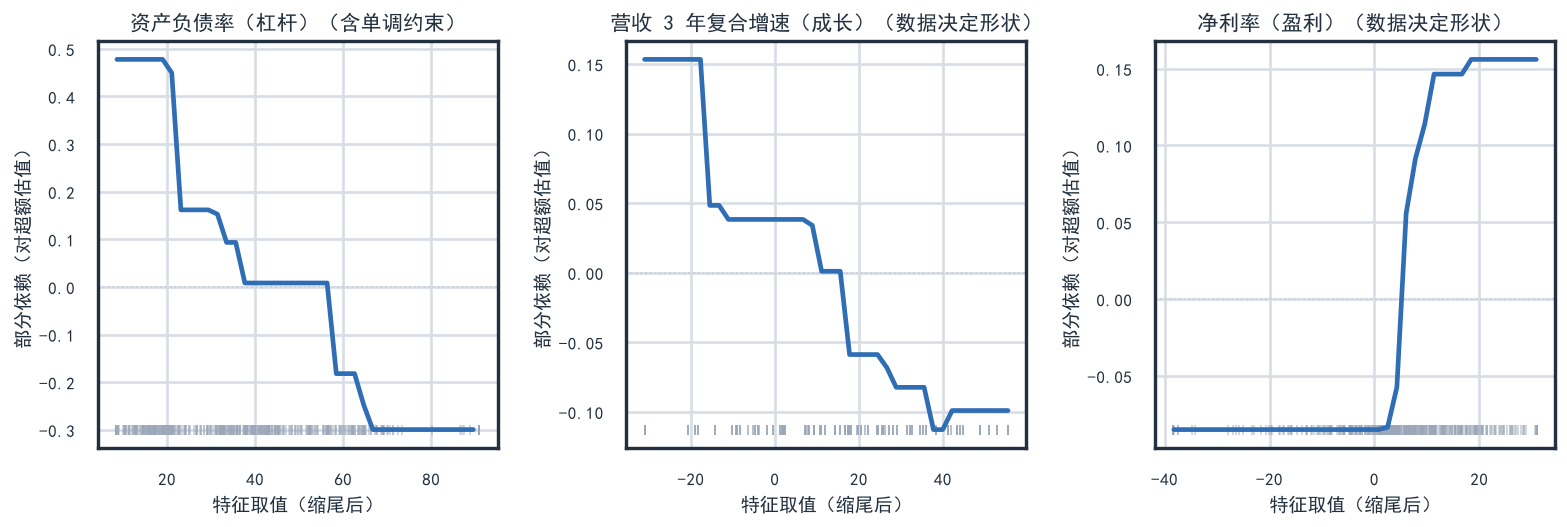
\includegraphics[width=\textwidth]{F_部分依赖.png}
\caption{三个核心特征对超额估值的部分依赖（梯度提升树）。曲线为固定其余特征、令该特征变化时的平均预测响应（已居中），底部竖线为实际观测分布。杠杆单调陡降（含单调约束）、成长单调递减（数据决定），与稳健结论一致；净利率呈阈值型（负利润区平坦、转正跃升），但该效应未通过稳健性检验。}
\label{fig:pdp}
\end{figure}

\section{白盒与黑盒的方向对照}
SHAP 只给重要性、不给方向。把梯度提升树（黑盒）对每个特征的经验方向，与白盒线性模型（第~\ref{ch:model}~章）的系数符号逐一对照，$17$ 个特征中有 $16$ 个方向一致（图~\ref{fig:wbbb}）：杠杆为负、成长为负、盈利为正，两个机理不同的模型给出同一套方向。这种一致使这张描述性地图的方向部分相当可靠。

\begin{figure}[htbp]
\centering
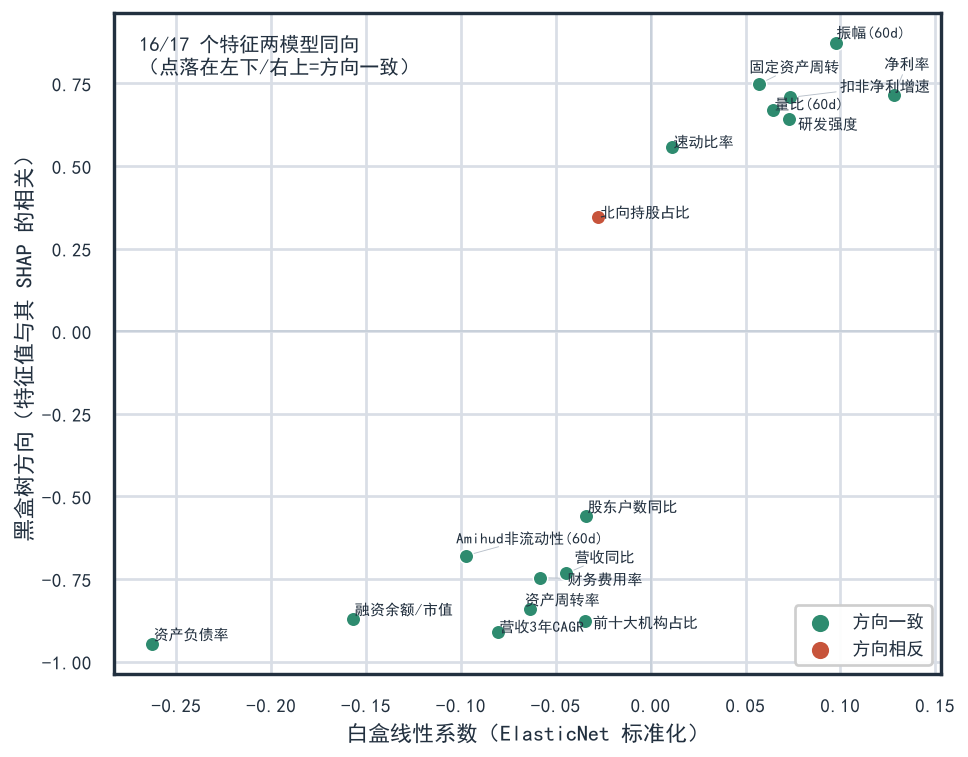
\includegraphics[width=0.78\textwidth]{F_白盒黑盒.png}
\caption{白盒与黑盒的方向对照。横轴为白盒线性模型的标准化系数，纵轴为黑盒树模型中特征值与其 SHAP 的相关（代表树的经验方向）。落在左下（同负）或右上（同正）象限即两模型同向；$17$ 个特征中 $16$ 个一致，仅北向持股占比一个例外。}
\label{fig:wbbb}
\end{figure}

\section{描述与推断的边界}
这张地图止于描述。特征间存在共线（第~\ref{ch:eda}~章），SHAP 会把贡献在相关特征之间分配，故单个特征的重要性数值不等于它的因果效应。本章确立的是“模型大致用了什么、哪些用得稳、方向是否自洽”；至于这些关联中哪些经得起少簇稳健检验、可被审慎地作因果性探讨，由下一章回答。

\chapter{稳健性与统计推断}\label{ch:robust}
本章是全报告推断的承重部分。前几章的机器学习只提供描述性地图；一个关联是否可信、可被审慎地作因果性探讨，由本章裁定。在仅 $14$ 家公司、有效独立簇约 $5$ 个的样本下，任何单一 $p$ 值都不足为凭。因此对每条预登记的核心关联，用五类探测不同失效模式的独立方法交叉检验——少簇稳健推断、设定稳健性、公司内识别、安慰剂证伪、留一家泛化——五者一致方认定可信。

\section{五方法三角验证矩阵}
三条预登记关联的检验结果汇于表~\ref{tab:tri}。两条关联——低杠杆溢价与成长折价——在五类方法下全部通过：点估计方向一致，少簇稳健推断（野自助、CR2、Romano--Wolf 多重校正）一致拒绝零效应，贝叶斯多层模型的 $95\%$ 可信区间不含零，公司内估计符号不变，安慰剂检验拒绝“随机也能得到同样强度”。盈利对估值的假设则相反：除点估计符号为正外，其余检验全部不显著，公司内估计甚至变号——它通不过严格检验，列为存疑。

\begin{table}[htbp]
\caption{三条预登记核心关联的五方法三角验证。各列为相互独立、各探不同失效模式的检验：野自助（少簇 wild cluster bootstrap 的 $p$）、CR2 稳健标准误（括号内为 Bell--McCaffrey 自由度）、Romano--Wolf 多重比较校正的 $p$、贝叶斯多层模型 $95\%$ 可信区间、公司内固定效应系数、安慰剂（随机置换）的 $p$。绿底为通过、红底为未过；判定列为通过的方法类数。}
\label{tab:tri}
\footnotesize
\renewcommand{\arraystretch}{1.55}
\setlength{\tabcolsep}{4pt}
\begin{tabular*}{\textwidth}{@{\extracolsep{\fill}}lccccccc@{}}
\toprule
\textbf{\color{brandblue}核心驱动} & \textbf{\color{brandblue}野自助} & \textbf{\color{brandblue}CR2 (df)} & \textbf{\color{brandblue}R--Wolf} & \textbf{\color{brandblue}贝叶斯 95\%} & \textbf{\color{brandblue}公司内} & \textbf{\color{brandblue}安慰剂} & \textbf{\color{brandblue}判定} \\
\midrule
低杠杆溢价 $(\beta\,{=}\,{-}0.52)$ & \cellcolor{okbg}$0.003$ & \cellcolor{okbg}$<\!0.001\,(5.0)$ & \cellcolor{okbg}$0.003$ & \cellcolor{okbg}$[{-}0.32,{-}0.19]$ & \cellcolor{okbg}${-}0.16$ & \cellcolor{okbg}$0.002$ & \cellcolor{okbg}\textbf{5/5} \\
成长折价 $(\beta\,{=}\,{-}0.17)$ & \cellcolor{okbg}$0.003$ & \cellcolor{okbg}$0.027\,(3.8)$ & \cellcolor{okbg}$0.005$ & \cellcolor{okbg}$[{-}0.24,{-}0.09]$ & \cellcolor{okbg}${-}0.17$ & \cellcolor{okbg}$0.002$ & \cellcolor{okbg}\textbf{5/5} \\
盈利溢价 $(\beta\,{=}\,{+}0.11)$ & \cellcolor{nobg}$0.41$ & \cellcolor{nobg}$0.49\,(4.5)$ & \cellcolor{nobg}$0.41$ & \cellcolor{nobg}$[{-}0.09,{+}0.01]$ & \cellcolor{nobg}${-}0.05$ & \cellcolor{nobg}$0.78$ & \cellcolor{nobg}\textbf{1/5} \\
\bottomrule
\end{tabular*}
\end{table}

\section{公司内识别}
把识别建立在公司内变异上，可剔除公司间恒定差异（行业地位、商业模式）造成的混淆。表~\ref{tab:tri} 的“公司内”一列即剔除这些差异后的系数。成长折价在公司内仍为 ${-}0.17$、与混合估计几乎一致，说明它来自同一家公司不同时期的内部变化，而非公司间的选择性差异。低杠杆溢价在公司内仍为负、符号稳健；但在同时吸收公司与年度变异的双向固定效应下，其幅度收窄、显著性减弱——这与杠杆本身是一项公司间相对稳定的特征相符：它刻画的更多是公司之间、而非同一公司逐季的估值差异。对低杠杆另做领先--滞后检验，“过去的杠杆 $\to$ 当期估值”的关系强于反向，反向因果不构成主要解释。

\section{安慰剂与设定曲线}
安慰剂检验最为直观（图~\ref{fig:placebo}）：把公司与特征的对应关系随机打乱、破坏真实链接后重新估计，得到一条“随机也能产生多大效应”的零分布。低杠杆与成长的实际效应都落在该零分布的尾部（$p=0.002$），随机重排几乎不可能产生这么强的关系；而盈利的实际效应恰落在分布中央（$p=0.78$），与随机不可区分。

\begin{figure}[htbp]
\centering
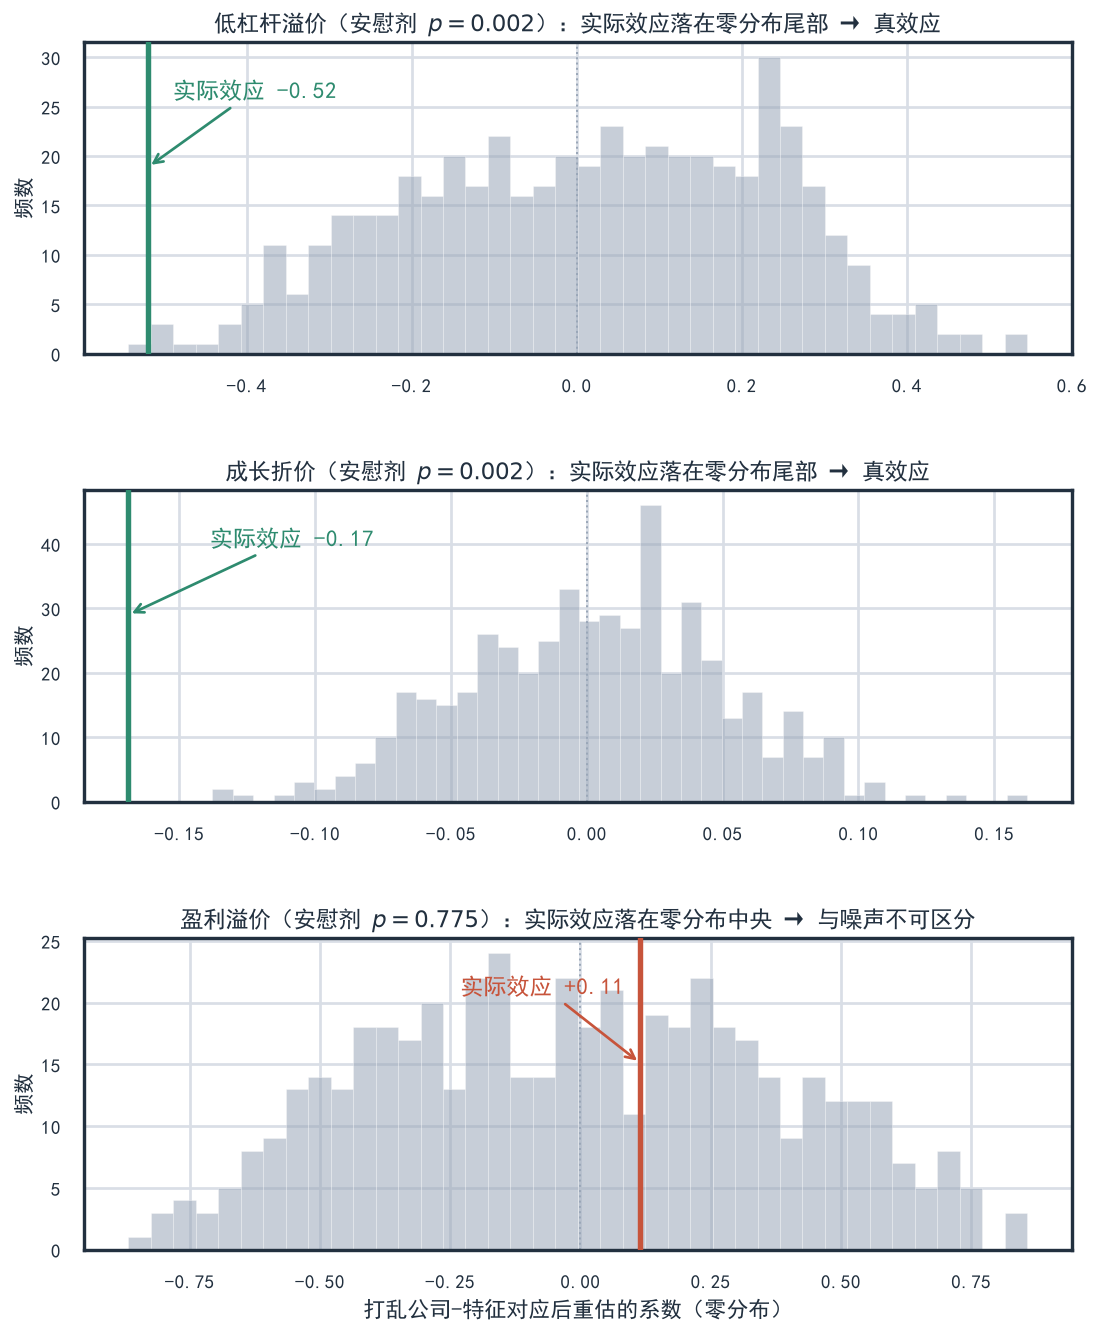
\includegraphics[width=0.80\textwidth]{F_安慰剂.png}
\caption{安慰剂检验。灰色直方图为打乱公司--特征对应后重估的系数零分布，竖线为实际效应。低杠杆（上，$-0.52$）与成长（中，$-0.17$）落在零分布尾部，是真效应；盈利（下，$+0.11$）落在分布中央，与噪声不可区分。}
\label{fig:placebo}
\end{figure}

设定稳健性从另一面佐证（图~\ref{fig:speccurve}）：把两条核心驱动放到一组合理设定（增减固定效应、增减控制变量、剔除最短样本或研究主体、不同缩尾档位）下逐一重估，成长折价在全部 $8$ 种设定下都为负且显著，低杠杆溢价在 $11$ 种设定中有 $10$ 种为负且显著，唯一例外正是上节所述的双向固定效应。

\begin{figure}[htbp]
\centering
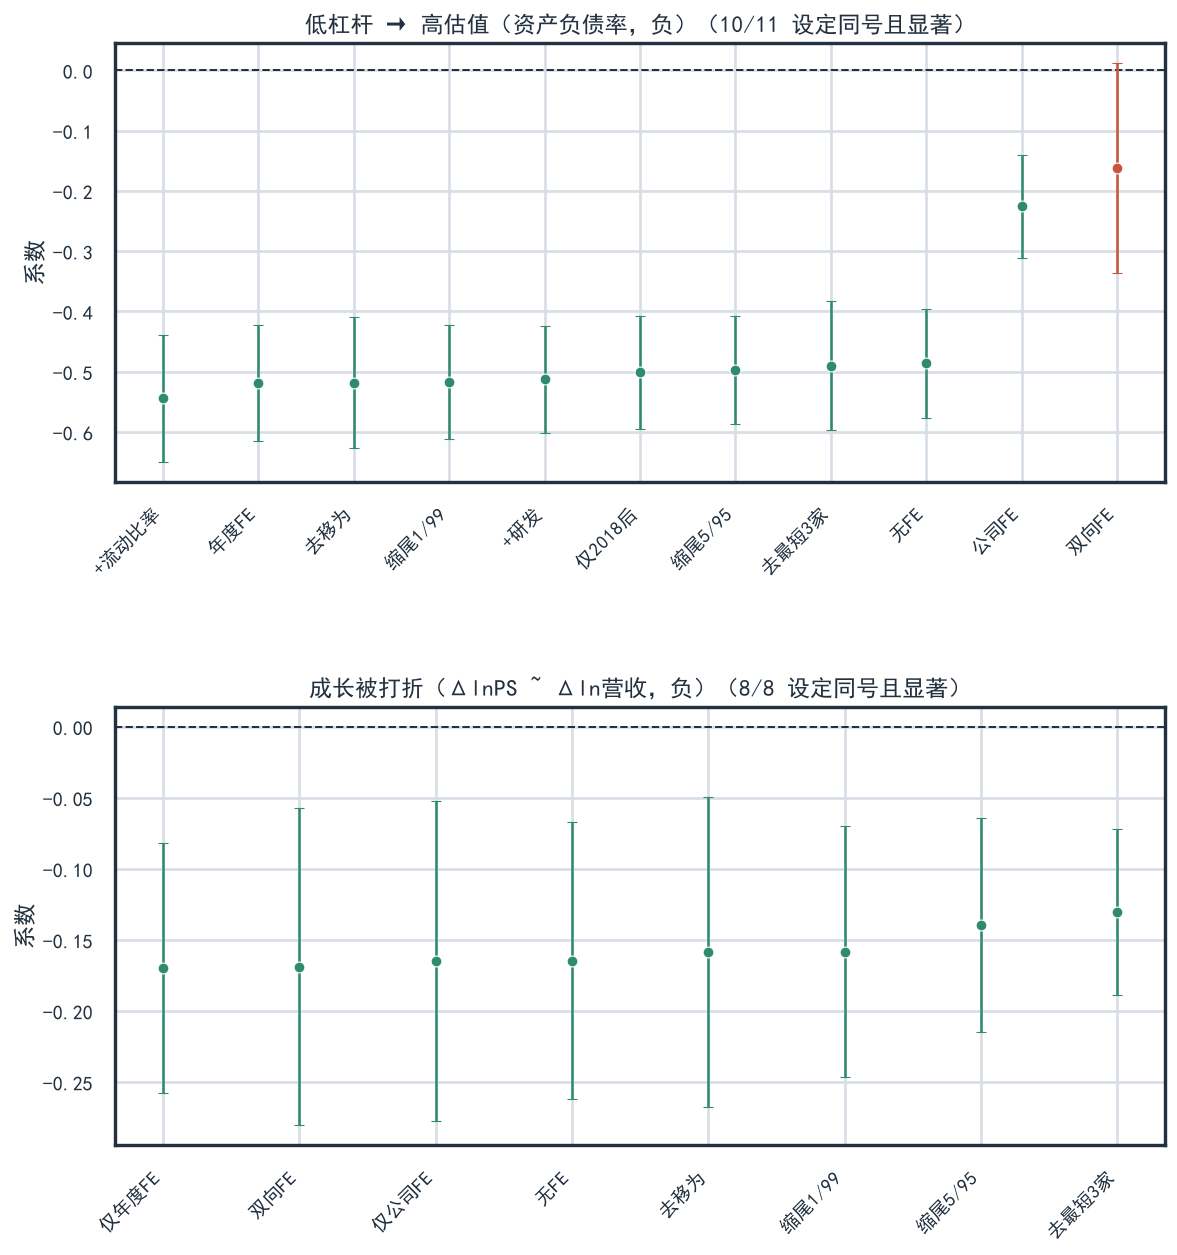
\includegraphics[width=0.78\textwidth]{F_设定曲线.png}
\caption{两条核心驱动的设定曲线。每个点为一种设定下的系数估计，竖线为按公司聚类的 $95\%$ 区间；绿色为同号且显著、红色为否，横虚线为零。上：低杠杆溢价（$10/11$ 设定为负且显著，例外为双向固定效应）；下：成长折价（$8/8$ 设定为负且显著）。}
\label{fig:speccurve}
\end{figure}

\chapter{结论}\label{ch:conclusion}
本报告以恒等分解为骨架、以面板与少簇稳健推断为主干，对 $14$ 家纯模组与终端公司的超额估值做了系统的解释性归因。三条预登记驱动的最终判定汇于图~\ref{fig:forest}：在标准化尺度上，资产负债率与超额估值呈稳健负相关（$\beta\approx-0.52$），营收增长对估值倍数同样为负（$\beta\approx-0.17$），二者的 Bell--McCaffrey $95\%$ 区间均不含零、且通过全部五类稳健性检验；净利率（剥离营收机械相关后）的偏效应区间宽跨零，未通过检验。由此得到两条确证的全域规律、与一条未获稳健支持的先验。

\begin{figure}[htbp]
\centering
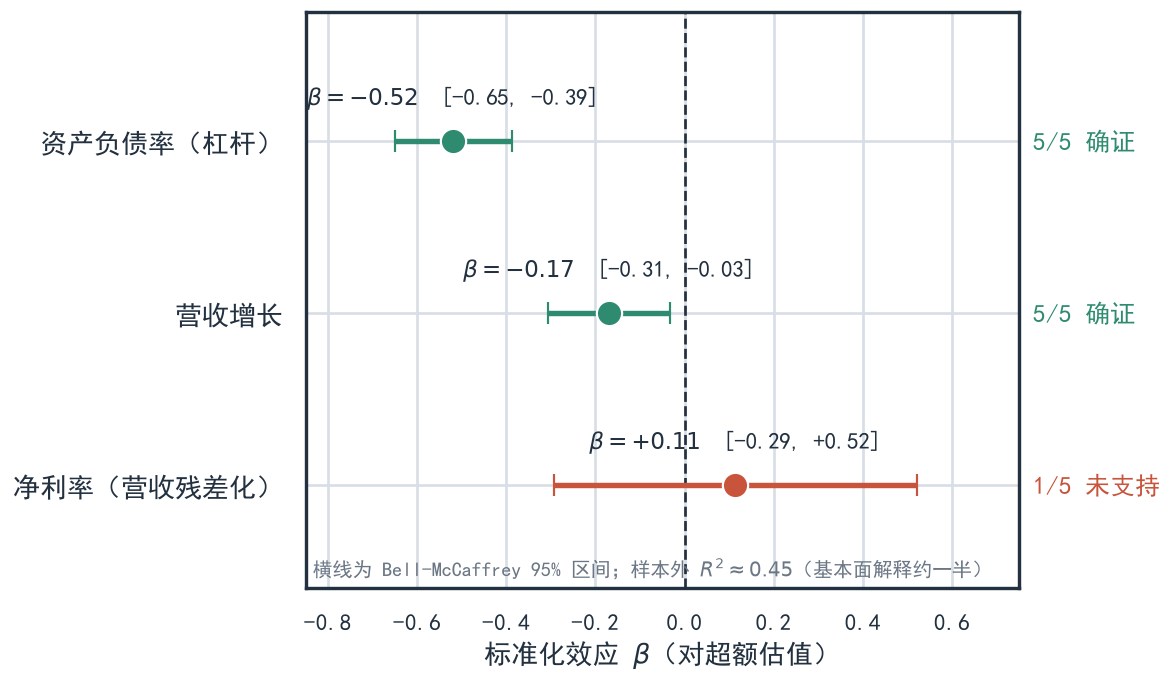
\includegraphics[width=\textwidth]{F_森林图.png}
\caption{三条核心驱动对超额估值的标准化效应汇总。点为 $\beta$，横线为 Bell--McCaffrey $95\%$ 区间，颜色与右栏标注五方法判定。资产负债率与营收增长的区间不含零、五法确证（绿）；净利率区间宽跨零、未获支持（红）。竖虚线为零效应。}
\label{fig:forest}
\end{figure}

\section{全域规律}
第一条是\textbf{低杠杆溢价}：负债率越低、超额估值越高；该关系在公司内估计中符号不变、在领先--滞后检验中以“杠杆 $\to$ 估值”为主导方向，是本样本中证据最强的驱动。第二条是\textbf{成长折价}：营收扩张伴随市销率倍数的系统性压缩，方向与“规模提升估值”的常见先验相反——在这一赛道，市场对单纯的规模扩张给予折价而非溢价。未获稳健支持的是\textbf{盈利溢价}：净利率对超额估值无稳健偏效应、公司内估计变号；且该检验功效不足（详见第~\ref{ch:limitations}~章），故判为非可靠驱动、而非已证明为零，不纳入解释集。解释力同时有明确边界：模型对未参与训练公司的样本外 $R^2\approx0.45$，即基本面只解释了跨公司估值差异的约一半，其余约一半为与基本面正交的特异与情绪成分。

\section{移为通信诊断}
就研究主体移为通信而言，其超额估值 $+0.70$ 可分解为基本面可解释的约 $+0.34$（占 $49\%$）与基本面解释不了的“情绪缺口”约 $+0.36$（占 $51\%$）。前者主要来自其显著低于同业的杠杆——这是移为在本模型下唯一稳健的估值优势来源；后者与基本面正交，更易随市场预期回摆。换言之，移为约一半的估值溢价有基本面支撑、可持续，另一半是脆弱的、模型之外的成分。

\section{决策剪枝}
把上述判定整理为决策含义，须区分“通过稳健性检验、可纳入解释”与“未通过、应从解释集剔除”的驱动，并标注其可操作性（表~\ref{tab:prune}）。唯一兼具稳健证据与公司可操作性的是杠杆；成长折价虽稳健、却非可正向操作的杠杆（增长本身不应停止）；盈利则无证据支撑。

\begin{table}[htbp]
\caption{驱动的决策剪枝。一致性为五方法中通过的类数；标准化效应为对超额估值的 $\beta$；操作性指该驱动是否为公司可正向调节的协变量。}
\label{tab:prune}
\footnotesize
\renewcommand{\arraystretch}{1.5}
\setlength{\tabcolsep}{5pt}
\begin{tabularx}{\textwidth}{@{}llllX@{}}
\toprule
\textbf{\color{brandblue}驱动} & \textbf{\color{brandblue}一致性} & \textbf{\color{brandblue}标准化效应} & \textbf{\color{brandblue}操作性} & \textbf{\color{brandblue}统计学含义} \\
\midrule
资产负债率 & \cellcolor{okbg}5/5 & $-0.52$ & 公司可控协变量 & 与超额估值稳健负相关、公司内符号不变；属观测性关联、未达因果识别，不可读作精确弹性 \\
营收增长 & \cellcolor{okbg}5/5 & $-0.17$ & 非正向操作项 & 倍数压缩为本样本的系统性定价特征，与“规模溢价”先验相反 \\
净利率（残差化） & \cellcolor{nobg}1/5 & $+0.11$ (n.s.) & --- & 偏效应不显著（WCB $p{=}0.41$）、公司内变号；功效不足，未获稳健支持 \\
特异/情绪成分 & --- & $\approx\!50\%$ 残差方差 & 不可解释 & 与基本面正交（$1-R^2_{\text{oos}}$），构成模型之外的不确定性敞口 \\
\bottomrule
\end{tabularx}
\end{table}

\section{主张的边界}
最后明确本报告主张的边界。这些关联建立在观测数据上——尽管经公司内识别、领先--滞后与安慰剂检验层层收窄，仍不等同于随机试验意义上的因果，其量级不应外推为精确弹性；解释力的上限约为一半，情绪与特异成分在模型之外；识别所依赖的有效独立簇约 $5$ 个，结论为量级判断而非精确点估计。在这些边界之内，本报告确证了两条全域规律、对一条流行先验未获稳健支持、并给出了移为估值的结构分解——这是 $14$ 家小样本经多方法交叉验证后能稳健支撑的结论。

\chapter{局限与有效性威胁}\label{ch:limitations}
任何基于 $14$ 家公司观测数据的解释性研究都面临若干效度威胁。本章把主要威胁逐一列出，交代研究设计已采取的缓解与未能消除的残余风险（表~\ref{tab:threats}），最后界定它们对结论的影响范围。

\begin{table}[htbp]
\caption{主要有效性威胁、设计缓解与残余风险。性质栏对应三角验证的推断/设定/识别/外部效度/泛化五维。}
\label{tab:threats}
\footnotesize
\renewcommand{\arraystretch}{1.45}
\setlength{\tabcolsep}{5pt}
\begin{tabularx}{\textwidth}{@{}llXX@{}}
\toprule
\textbf{\color{brandblue}威胁} & \textbf{\color{brandblue}性质} & \textbf{\color{brandblue}设计缓解} & \textbf{\color{brandblue}残余风险} \\
\midrule
有效独立簇约 $5$ 个 & 推断 & 野自助、CR2 与 Bell--McCaffrey 自由度、Romano--Wolf、贝叶斯多层五法并用 & 结论为量级判断，非精确点估计 \\
生成回归量 $Y$（一阶段设定依赖） & 设定 & 一阶段剥离规模与年度固定效应、特征缩尾 & 二阶段未传播一阶段估计误差，且依赖一阶段设定正确 \\
观测性关联 & 识别 & 公司内固定效应、领先--滞后、安慰剂检验 & 非随机试验意义上的因果 \\
时段与市场环境稳定性 & 外部效度 & 年度固定效应吸收估值水平漂移 & 定价关系斜率随环境漂移未建模；样本限在册公司，对退市/未上市/异质业务外推受限 \\
非平衡面板与短历史 & 泛化 & 留一家、留时段外推验证 & 次新股外推方差大 \\
\bottomrule
\end{tabularx}
\end{table}

\section{推断与设定}
在推断层面，最根本的约束是有效独立簇仅约 $5$ 个：样本虽有 $14$ 家公司、$483$ 个观测，但同业间存在共同的行业冲击，真正独立的信息单元远少于观测数。本报告以五类少簇稳健方法应对，并一律将结论表述为量级而非精确点估计。在设定层面，目标 $Y$ 是第一阶段回归（市销率对规模与年度固定效应）的残差，属生成回归量——其构造依赖第一阶段设定的正确性，且第二阶段未传播第一阶段的估计误差；缩尾与稳健标准误缓解了部分影响，但这一依赖无法完全消除。

\section{统计功效与可检测效应}
小样本的另一面是检验功效：一个未达显著的关联，可能是真无效应，也可能是样本太小、检验无力分辨。为区分二者，对每条核心驱动用其聚类稳健标准误，计算可检出的最小效应（MDE，双侧 $\alpha=0.05$、功效 $80\%$）与检出其观测效应的功效（表~\ref{tab:power}）。低杠杆与成长的标准误小、功效近 $1$，其结论是在充分功效下成立的。盈利则不同：其标准误约为另两者的三倍，仅能可靠检出大于约 $0.43$ 的效应，而观测效应仅 $0.11$、对应功效约 $0.11$。

因此“盈利无估值驱动”应理解为\textbf{未获稳健支持、且检验功效不足}——数据既未发现盈利溢价，也无力排除一个中等大小的效应；结合其公司内估计变号、安慰剂落于零分布中央，本报告将其归为非可靠驱动，而非已证明严格为零。这一区分对决策同样重要：它意味着“盈利不影响估值”是一个谨慎的工作判断，而非可外推的定论。

\begin{table}[htbp]
\caption{三条核心驱动的统计功效。SE 为聚类稳健标准误；MDE@80\% 为双侧 $\alpha=0.05$、功效 $80\%$ 下可检出的最小标准化效应；末列为检出各自\emph{观测}效应的功效。}
\label{tab:power}
\footnotesize
\renewcommand{\arraystretch}{1.35}
\begin{tabular*}{\textwidth}{@{\extracolsep{\fill}}lcccc@{}}
\toprule
\textbf{\color{brandblue}驱动} & \textbf{\color{brandblue}$\beta$} & \textbf{\color{brandblue}SE} & \textbf{\color{brandblue}MDE@80\%} & \textbf{\color{brandblue}检出观测效应的功效} \\
\midrule
低杠杆 & $-0.52$ & $0.05$ & $0.14$ & $\approx 1.00$（充分） \\
成长 & $-0.17$ & $0.05$ & $0.13$ & $0.94$（充分） \\
盈利 & $+0.11$ & $0.15$ & $0.43$ & $0.11$（功效不足） \\
\bottomrule
\end{tabular*}
\end{table}

\section{识别与因果}
全部关联建立在观测数据上。公司内固定效应剔除了公司间恒定的混淆，领先--滞后检验显示主导方向为“特征 $\to$ 估值”，安慰剂检验排除了随机产生同等强度的可能；这些设计层层收窄了替代解释，但都不等同于随机试验。因此本报告的结论以稳健关联陈述，而非因果效应，其量级也不应外推为精确弹性。

\section{外部效度与泛化}
在外部效度层面有两点须界定。其一是时段与市场环境：样本期跨 $2009$ 至 $2026$ 年、覆盖牛熊与风格切换等多个环境，年度固定效应吸收了各年估值水平的整体漂移，但并未建模定价关系\emph{斜率}随环境的变化——例如市场对成长的折价幅度在不同情绪周期可能不同。因此本报告的系数应理解为样本期内的平均关系，而非任一特定时点或未来环境下的恒定值。其二是样本构成：$14$ 家公司均为截至成稿仍在上市者，已退市或从未上市的同类公司不在其中，构成幸存者选择；若退市公司的估值--基本面关系系统性不同，则本报告的横截面规律对全体（含已消失）公司的外推会有偏。

在泛化层面，非平衡面板中次新股（如博实结仅 $9$ 期）历史极短，留一家外推时模型对其几乎无同公司历史可借，外推方差较大，涉及这些公司的个体结论须谨慎；而全域规律因汇集全部 $14$ 家、受单家影响有限，相对稳健。

\section{多重比较与研究者自由度}
另一类威胁来自分析过程本身的灵活性。本报告检验的三条核心假设是预登记的——方向与口径在建模前即已确定，而非从数据中挑选；跨假设的多重比较以 Romano--Wolf 方法校正，压低了多重检验下偶然显著的风险。但更广义的研究者自由度仍然存在：特征工程的口径、缩尾的档位、模型族与正则强度的选择都包含判断。本报告以三条原则约束这一空间——所有预处理与选择服从防泄漏与防过拟合的事先规则、关键选择在嵌套交叉验证的每折内部独立重做、全流程在固定种子下可复现（附录~\ref{app:repro}）——但这些措施只能压缩、不能消灭分析灵活性带来的不确定性。读者应把本报告的结论理解为“在一套事先声明、全程可复现的分析下成立”，而非唯一可能的分析路径下的唯一结果。

\section{威胁的影响范围}
这些威胁均已如实披露，并通过研究设计与多方法交叉验证收敛到可控范围。它们限定了本报告主张的精度与适用域——量级而非点估计、关联而非因果、样本期平均而非跨环境恒定——但不动摇核心结论：在 $14$ 家小样本、五类方法一致的前提下，低杠杆溢价与成长折价稳健成立，盈利溢价不成立。

\appendix
\chapter{可复现性}\label{app:repro}
本附录交代运行环境、数据接口、随机种子与复现步骤，使全部结果可被独立重跑。

\section{运行环境}
分析在 Python $3.12$ 下完成，核心依赖为 \texttt{lightgbm}（梯度提升树）、\texttt{scikit-learn}（L1 选择与交叉验证）、\texttt{statsmodels} 与自实现的少簇稳健推断、\texttt{numpyro}（贝叶斯多层模型）、\texttt{shap}（归因），以及 \texttt{numpy}/\texttt{pandas}/\texttt{scipy}。所有计算在固定随机种子下单机可复现，不依赖网络（数据已落盘）。

\section{数据接口}
进入模型的量化数据均来自 Tushare Pro，接口与用途见表~\ref{tab:tushare}；各接口返回均带公告日时间戳，按公告日以最近可得值对齐至各报告期。

\begin{table}[htbp]
\caption{Tushare Pro 数据接口清单。}
\label{tab:tushare}
\footnotesize
\renewcommand{\arraystretch}{1.35}
\begin{tabular*}{\textwidth}{@{\extracolsep{\fill}}lll@{}}
\toprule
\textbf{\color{brandblue}用途} & \textbf{\color{brandblue}接口} & \textbf{\color{brandblue}主要字段} \\
\midrule
财务指标 & \texttt{fina\_indicator} & 利润率、回报率、周转、杠杆、成长 \\
三大报表 & \texttt{income / balancesheet / cashflow} & 营收、利润、资产负债、现金流 \\
每日指标 & \texttt{daily\_basic} & 总市值、市销率 PS、换手率、量比 \\
主营业务构成 & \texttt{fina\_mainbz} & 海外/分地区收入 \\
沪深股通持股 & \texttt{hk\_hold} & 北向持股占比 \\
融资融券明细 & \texttt{margin\_detail} & 融资余额 \\
个股资金流向 & \texttt{moneyflow} & 主力净流入 \\
股东户数 & \texttt{stk\_holdernumber} & 股东户数 \\
前十大流通股东 & \texttt{top10\_floatholders} & 机构持股集中度 \\
\bottomrule
\end{tabular*}
\end{table}

\section{随机种子与复现步骤}
全部模型与重采样使用固定种子 $\text{RNG}=0$：梯度提升树、L1 的 \texttt{LassoCV}、嵌套交叉验证、自助与置换均以此初始化。重采样次数固定为——三角验证的野自助与置换 $B=599$、成对自助稳定性 $B=400$、嵌套交叉验证每折内调参 $40$ 次。复现按以下顺序运行：\texttt{build\_valuation\_model.py}（建模、L1 选择、SHAP、留一家/留时段评估）、\texttt{verify\_drivers\_triangulation.py}（五方法三角验证）、\texttt{build\_stability\_bootstrap.py}（稳定性区间）、\texttt{build\_nested\_cv.py}（嵌套交叉验证）、\texttt{build\_ch8\_diagnostics.py}（复杂度最优区间与解释力阶梯）。各脚本将结果写入 JSON；在固定种子下重复运行两次产物逐字节一致。

\section{时点对齐}
所有特征按公告日（而非报告期期末）对齐，以杜绝前视偏误：在每个“公司—报告期”观测点，仅使用截至该报告期对齐日已公告、已可得的最近一期数据。季度财务数据按其实际披露日填入——年报通常在次年一季度披露，故某年年报的指标只在其披露日之后的报告期才进入面板；市场类特征（换手率、振幅、北向持股、融资余额等）以对齐日前 $60$ 个交易日的窗口计算，不含对齐日之后的任何行情。目标变量也仅由当期及历史数据构造。任何需要使用未来信息才能计算的字段均不纳入候选集。这一对齐使面板在每个时点都只含“当时可得”的信息，模型的样本外评估（留时段、留一家）因而是对真实可操作信息集的外推。

\chapter{模型卡与数据表}\label{app:modelcard}
本附录以模型卡形式汇总模型的用途、设定、指标与局限，便于使用者快速判断其适用边界。

\section{模型卡}
\begin{table}[htbp]
\caption{估值归因模型卡。}
\label{tab:modelcard}
\footnotesize
\renewcommand{\arraystretch}{1.45}
\begin{tabularx}{\textwidth}{@{}lX@{}}
\toprule
\textbf{\color{brandblue}条目} & \textbf{\color{brandblue}内容} \\
\midrule
用途 & 解释 $14$ 家纯模组与终端公司的超额估值\emph{为何}在公司间与时间上不同；作描述性归因 \\
不适用 & 预测个股未来股价或收益；外推至样本外行业、退市/未上市公司；作精确因果效应或弹性 \\
目标变量 & 超额估值 $Y=\log(\text{PS})$ 剥离规模与年度固定效应后的残差，缩尾 $2/98$ \\
输入 & $42$ 个候选特征经 L1 选择保留 $17$ 个（定义见附录~\ref{app:datadict}） \\
主模型 & 深度受限梯度提升树（叶数 $\leq7$、树深 $\leq3$；仅资产负债率施加单调 $-1$ 约束） \\
白盒对照 & 无约束 ElasticNet 线性模型，用于方向交叉验证 \\
推断主干 & 面板/公司内回归 + 五方法少簇稳健推断（见第~\ref{ch:robust}~章） \\
评估口径 & 仅报样本外（留一家、留时段）$R^2$；样本内仅作过拟合诊断 \\
局限 & 有效独立簇约 $5$；目标为生成回归量；关联非因果（详见第~\ref{ch:limitations}~章） \\
\bottomrule
\end{tabularx}
\end{table}

\section{关键超参与指标}
最终超参由按公司分组交叉验证在浅档网格内选定，主要解释力指标见表~\ref{tab:metrics2}。样本内与样本外的显著落差（$0.85$ 对约 $0.45$）正是只报样本外的理由；嵌套交叉验证将选择与调参全部移入折内后，留一家 $R^2$ 仍为 $0.45$，确认无选择性泄漏。

\begin{table}[htbp]
\caption{关键超参数与解释力指标。}
\label{tab:metrics2}
\footnotesize
\renewcommand{\arraystretch}{1.4}
\begin{tabular*}{\textwidth}{@{\extracolsep{\fill}}llll@{}}
\toprule
\multicolumn{2}{@{}l}{\textbf{\color{brandblue}超参数}} & \multicolumn{2}{l}{\textbf{\color{brandblue}解释力（$R^2$）}} \\
\midrule
叶节点数 & $4$ & 样本内 & $0.847$ \\
最大树深 & $2$ & 分组交叉验证 & $0.442$ \\
树的棵数 & $200$ & 留时段（OOT） & $0.497$ \\
学习率 & $0.05$ & 留一家（LOFO） & $0.454$ \\
L1 / L2 正则 & $2$ / $1$ & 嵌套交叉验证（留一家） & $0.452$ \\
行/列采样 & $0.6$ / $1.0$ & 未解释占比 & $\approx 0.55$ \\
\bottomrule
\end{tabular*}
\end{table}

这些指标共同界定了模型的可信使用方式。样本内 $R^2=0.85$ 仅反映对已知公司的拟合能力，不作为性能主张；真正衡量解释力的是样本外口径：分组交叉验证（留出整家公司）$0.44$、留时段 $0.50$、留一家 $0.45$，三者一致地指向“基本面解释约一半”。其中留时段略高于留一家，说明对未来时段的外推略易于对全新公司的外推，与样本内公司历史更长、时序结构更易学习相符。嵌套交叉验证把特征选择、缩尾与调参全部移入每折内部、各折独立重做 $40$ 次，留一家 $R^2$ 仍为 $0.45$、与主流程几乎一致，排除了选择性泄漏抬高指标的可能。未解释的约 $0.55$ 即与基本面正交的特异与情绪成分，其性质与边界详见第~\ref{ch:validation}~章。

\chapter{L1 特征选择明细}\label{app:l1}
本附录交代 L1 特征选择的方法，并给出被剔除的 $25$ 个特征的逐项明细。正文第~\ref{ch:select}~章对此有概述。

\section{选择方法}
特征选择以 L1 正则的 Lasso 完成，并把正则强度 $\alpha$ 的确定嵌入按公司分组的交叉验证（\texttt{LassoCV} 配合 GroupKFold，组为公司）：每折留出整家公司，在其余公司上拟合、在留出公司上评估，从而避免同一公司不同报告期之间的信息泄漏；$\alpha$ 取交叉验证误差最小处，对应非零系数的特征即被保留。选用 L1 而非逐步回归或方差膨胀因子逐项剔除，是因为在“特征数接近样本量一半、且存在多组高相关特征”的情形下，L1 能稳定地在每组冗余特征中择一保留、把其余压缩为零，与本问题的结构相符。在嵌套交叉验证与成对自助中，这一选择在每折/每次重抽内部独立重做，故下文的 $17$ 个为全样本选择结果，其逐特征稳定性另见可解释性一章。

\section{被剔除特征的两类}
在选定的 $\alpha$ 下，$42$ 个候选被压缩为 $17$ 个、剔除 $25$ 个，按其与最相关保留特征的相关系数 $r$ 分为两类（图~\ref{fig:l1}）。第一类是\textbf{高共线冗余}（$r\geq0.5$，共 $15$ 个）：信息已被某个保留特征覆盖，例如现金比率与速动比率相关 $0.98$、流动比率与速动比率 $0.90$、应收周转与资产周转率 $0.78$——同组保留其一即可，删除不损失独立信息。第二类是\textbf{弱信号}（$r<0.5$，共 $10$ 个）：与目标超额估值关联微弱，在保留特征之外不再贡献解释力，被 L1 惩罚归零。两类的共同点是删除后保留集所含信息不变——这也是后续 SHAP 与系数解读只在 $17$ 个保留特征上进行的依据。每个被删特征与其最相关保留特征的对应关系见图~\ref{fig:l1}：横条为二者相关系数 $r$，红色为高共线冗余、灰色为弱信号。

\begin{figure}[htbp]
\centering
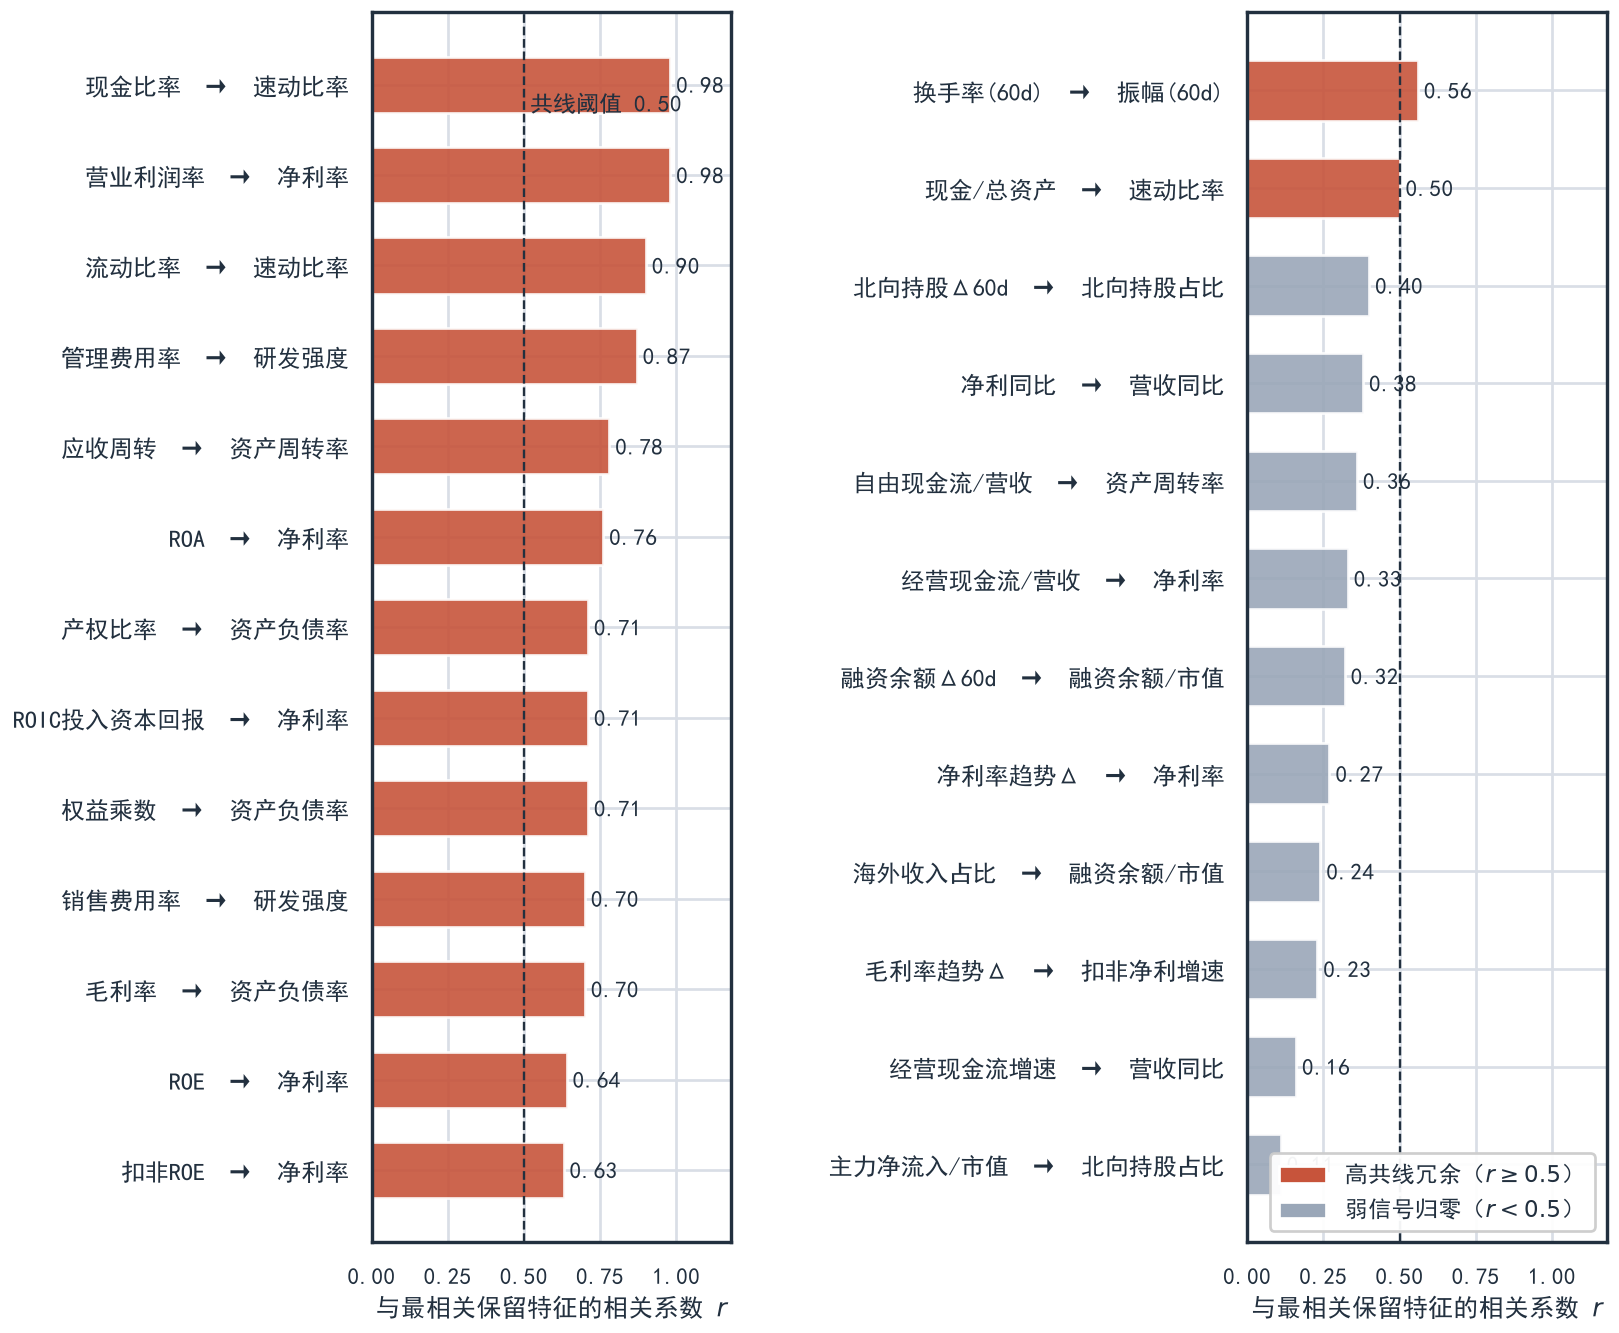
\includegraphics[width=\textwidth]{F9_L1特征选择剔除.png}
\caption{L1 特征选择剔除的 $25$ 个特征（按相关系数从高到低排列，左栏高、右栏低）。每行一个被删特征，箭头指向与它最相关的保留特征，横条为二者相关系数 $r$；红色为高共线冗余（$r\geq0.5$，如现金比率与速动比率 $0.98$），灰色为弱信号归零（$r<0.5$）。虚线为 $0.5$ 共线参考阈值。}
\label{fig:l1}
\end{figure}

\section{保留的 17 个特征}
最终进入模型的 $17$ 个特征横跨互补维度、彼此冗余度低：盈利（净利率）；运营效率（资产周转率、固定资产周转）；成长（营收同比、营收 $3$ 年 CAGR、扣非净利增速）；杠杆与流动性（资产负债率、速动比率）；费用与研发（研发强度、财务费用率）；市场流动性（量比、振幅、Amihud 非流动性，均取 $60$ 日窗口）；筹码与资金（股东户数同比、北向持股占比、融资余额/市值、前十大机构占比）。这一组合在第~\ref{ch:model}~章作为建模输入，其系数方向与稳定性分别由白盒线性模型（第~\ref{ch:model}~章）与成对自助稳定性区间（第~\ref{ch:interp}~章）刻画。值得注意的是，这 $17$ 个并非都稳健——稳定性分析显示，仅杠杆、成长与若干市场结构特征构成可靠的稳定核心，盈利类特征虽入选却在重抽中频繁进出。

\chapter{数据字典}\label{app:datadict}
本附录列出 $42$ 个候选特征的中文名、代码键、类别与计算口径。括注的代码键与复现脚本中的字段一一对应。比率类特征均以同期财务数据计算，市场类特征以报告期对齐日前 $60$ 个交易日的窗口计算。

\footnotesize
\renewcommand{\arraystretch}{1.3}
\begin{longtable}{@{}>{\raggedright\arraybackslash}p{3.9cm}>{\raggedright\arraybackslash}p{2.0cm}>{\raggedright\arraybackslash}p{8.5cm}@{}}
\toprule
\textbf{\color{brandblue}特征（代码键）} & \textbf{\color{brandblue}类别} & \textbf{\color{brandblue}定义与口径} \\
\midrule
\endfirsthead
\multicolumn{3}{@{}l}{\footnotesize（续表~\ref{app:datadict}）}\\
\toprule
\textbf{\color{brandblue}特征（代码键）} & \textbf{\color{brandblue}类别} & \textbf{\color{brandblue}定义与口径} \\
\midrule
\endhead
\bottomrule
\endfoot
净利率 (\texttt{\scriptsize f\_net\_margin}) & 盈利 & 净利润 / 营业收入 \\
毛利率 (\texttt{\scriptsize f\_gross\_margin}) & 盈利 & （营业收入 $-$ 营业成本）/ 营业收入 \\
营业利润率 (\texttt{\scriptsize f\_op\_margin}) & 盈利 & 营业利润 / 营业收入 \\
ROE (\texttt{\scriptsize f\_roe}) & 回报 & 净利润 / 净资产 \\
ROA (\texttt{\scriptsize f\_roa}) & 回报 & 净利润 / 总资产 \\
ROIC (\texttt{\scriptsize f\_roic}) & 回报 & 息税前利润$\times(1-$税率$)$ / 投入资本 \\
扣非 ROE (\texttt{\scriptsize f\_roe\_dt}) & 回报 & 扣非净利润 / 净资产 \\
资产周转率 (\texttt{\scriptsize f\_asset\_turn}) & 运营 & 营业收入 / 总资产 \\
应收周转 (\texttt{\scriptsize f\_ar\_turn}) & 运营 & 营业收入 / 应收账款 \\
固定资产周转 (\texttt{\scriptsize f\_fa\_turn}) & 运营 & 营业收入 / 固定资产 \\
营收同比 (\texttt{\scriptsize f\_rev\_yoy}) & 成长 & 营业收入较去年同期增速 \\
净利同比 (\texttt{\scriptsize f\_ni\_yoy}) & 成长 & 净利润较去年同期增速 \\
营收 3 年 CAGR (\texttt{\scriptsize f\_rev\_cagr3}) & 成长 & 营业收入三年复合增速 \\
扣非净利增速 (\texttt{\scriptsize f\_dt\_ni\_yoy}) & 成长 & 扣非净利润同比增速 \\
经营现金流增速 (\texttt{\scriptsize f\_ocf\_yoy}) & 成长 & 经营活动现金流净额同比增速 \\
经营现金流/营收 (\texttt{\scriptsize f\_ocf\_to\_rev}) & 现金流 & 经营活动现金流净额 / 营业收入 \\
自由现金流/营收 (\texttt{\scriptsize f\_fcf\_to\_rev}) & 现金流 & （经营现金流 $-$ 资本开支）/ 营业收入 \\
现金/总资产 (\texttt{\scriptsize f\_cash\_to\_assets}) & 现金流 & 货币资金 / 总资产 \\
资产负债率 (\texttt{\scriptsize f\_debt\_to\_assets}) & 杠杆 & 总负债 / 总资产 \\
权益乘数 (\texttt{\scriptsize f\_equity\_mult}) & 杠杆 & 总资产 / 净资产 \\
产权比率 (\texttt{\scriptsize f\_debt\_to\_eqt}) & 杠杆 & 总负债 / 净资产 \\
流动比率 (\texttt{\scriptsize f\_current\_ratio}) & 流动性 & 流动资产 / 流动负债 \\
速动比率 (\texttt{\scriptsize f\_quick\_ratio}) & 流动性 & （流动资产 $-$ 存货）/ 流动负债 \\
现金比率 (\texttt{\scriptsize f\_cash\_ratio}) & 流动性 & 货币资金 / 流动负债 \\
研发强度 (\texttt{\scriptsize f\_rd\_intensity}) & 费用 & 研发支出 / 营业收入 \\
销售费用率 (\texttt{\scriptsize f\_saleexp\_ratio}) & 费用 & 销售费用 / 营业收入 \\
管理费用率 (\texttt{\scriptsize f\_adminexp\_ratio}) & 费用 & 管理费用 / 营业收入 \\
财务费用率 (\texttt{\scriptsize f\_finaexp\_ratio}) & 费用 & 财务费用 / 营业收入 \\
净利率趋势 $\Delta$ (\texttt{\scriptsize d\_net\_margin}) & 趋势 & 净利率近若干期的变化量 \\
毛利率趋势 $\Delta$ (\texttt{\scriptsize d\_gross\_margin}) & 趋势 & 毛利率近若干期的变化量 \\
海外收入占比 (\texttt{\scriptsize f\_overseas\_share}) & 海外 & 海外营业收入 / 总营业收入 \\
换手率 (60d) (\texttt{\scriptsize liq\_turn}) & 流动性·市场 & 近 $60$ 交易日平均换手率 \\
量比 (60d) (\texttt{\scriptsize liq\_volratio}) & 流动性·市场 & 近 $60$ 交易日平均量比 \\
振幅 (60d) (\texttt{\scriptsize liq\_amplitude}) & 流动性·市场 & 近 $60$ 交易日平均日振幅 \\
Amihud 非流动性 (60d) (\texttt{\scriptsize liq\_amihud}) & 流动性·市场 & 近 $60$ 日 $|$收益$|$/成交额 的均值 \\
股东户数同比 (\texttt{\scriptsize chip\_holder\_yoy}) & 筹码 & 股东户数较去年同期变化 \\
北向持股占比 (\texttt{\scriptsize nf\_north\_ratio}) & 资金 & 沪深股通持股 / 流通股本 \\
北向持股 $\Delta$60d (\texttt{\scriptsize nf\_north\_chg}) & 资金 & 北向持股占比近 $60$ 日变化 \\
融资余额/市值 (\texttt{\scriptsize nf\_margin\_ratio}) & 资金 & 融资余额 / 总市值 \\
融资余额 $\Delta$60d (\texttt{\scriptsize nf\_margin\_chg}) & 资金 & 融资余额近 $60$ 日变化 \\
前十大机构占比 (\texttt{\scriptsize nf\_inst\_top10}) & 筹码 & 前十大流通股东中机构持股占比 \\
主力净流入/市值 (\texttt{\scriptsize nf\_mf\_net}) & 资金 & 主力资金净流入 / 总市值 \\
\end{longtable}
\normalsize

\end{document}
